\chapter{Differential networks reveal the dynamics of animal pests and disease co-occurrences}

\subsection{Introduction}
Rice (\textit{Oryza sativa}) is a major crop in South and Southeast Asian. Generally, rice farmers cultivate 2 rice crops per year, with the typical seasonal crop cycles or rotations being rice-rice-fallow or rice-rice-secondary crops (corn, soybean, peanut). The Food and Agriculture Organization of the United Nations (FAO) estimates that approximately 70 percent of total lowland rice area produces 2 rice crops each year. The first crop is cultivated in the wet season, while another is in the dry season. The important role of seasonal cropping in the temporal dynamics of animal pests and diseases has been studied under farmers field survey in South and Southeast Asia by the use of multivariate techniques \citet{Savary_2000_Characterization, Willocquet_2008_Simulating}. The previous studies showed that Injuries profiles (the combination of injuries) differ from season to season in term of weather pattern. In the dry season, crop losses were lower than in the wet season. A previous study based on surveys done in farmers’ rice fields in the region of lowland rice were shown to be strongly associated with injury profiles.

In the previous chapter, the co-occurrence networks to yield co-occurrence networks, a methodological approach which has already proved fruitful in a variety of different applications.  Plant injuries caused by pests maybe affect yield production. Therefore, in this chapter, I attempted to characterize the patterns of rice injuries by studying the changes in the co-occurrence patterns of rice injuries (\textit{e.g} disease incidence, animal pest injury incidence) at different yield levels.

Differential network analysis aims to compare the connectivity of two nodes at 2 different conditions. As demonstrated by several studies, differential networks can identify important nodes implicated in my fields, and also provide critical novel insights not obtainable using other approaches. In this work, I explore the the properties of network of a complex association of rice injuries at different yield levels. Elucidating the rice injuries association represents a key challenge, not only for achieving a deeper understanding of injury association (injury profiles) but also for identifying the unique association. Given that the injury association is governed by a complex network of injuries association, it seems natural to explore network properties which may help elucidate some of different association presenting in the different seasons.

In this chapter, I employ a differential network topology method to examine the co-occurrence relationships of rice injuries from survey data. I use graph theory methods to examine the topological feature dynamic of a co-occurrence network corresponding to different seasons, and production environments. The co-occurrence networks were built from differentially co-occurring injuries. I extract significantly differential co-occurring injuries from co-occurrence networks, which represent different seasons, to identify which injuries that may be involved specifically curtain season. I postulate that these selected injuries may contribute to the difference in the co-occurrence patterns in different season. Furthermore, I identified the injuries associated with yield from networks at different yield levels. Finally, I suggest key injuries that may contribute to yield reduction under a curtain production environment. The goal is to leverage insights to better understand the rice injury co-occurrence that may contribute to pest management development.

\subsection{Materials and Methods}

\textbf{Differential co-occurrence network construction}

The survey data were pre-processed by using methods described in the previous chapter. Subsequently, I applied the method proposed by \citet{Fukushima_2013_Diffcorr} to identify differentially co-occurrence links. The difference of co-occurrence of injury $x$ and $y$ between two conditions ($A$ and $B$) was quantified by Fisher's $z$-test.
 
For the pair of $x$ injury and $y$ injury, I denoted the correlation coefficient based on Spearman's correlation coefficient by $r_{xy}^A$ and $r_{xy}^A$ in networks of condition $A$ and condition $B$, respectively. To test whether the 2 correlation coefficients were significantly different, correlation coefficients for each of the 2 conditions, $r_{xy}^A$ and $r_{xy}^B$, were transformed into $Z_{xy}^A$ and $Z_{xy}^B$, respectively.


The Fisher's transformation of coefficient $r_{xy}^A$ is defined by
\begin{equation}
\label{eq:zvalue}
Z_{xy} = \frac{1}{2} \log\left[{\frac{1 + r_{xy}}{1 - r_{xy}}}\right]
\end{equation}

Next, The $p$-value of the difference in $Z_{xy}$ values was calculated using the standard normal distribution.

\begin{equation}
\label{eq:pofz}
p(Z\geq \left | \frac{Z_{xy}^A - Z_{xy}^B}{\sqrt{\frac{1}{N_{A}-3}+ \frac{1}{N_{A}-3}}} \right |
\end{equation}

Next, The $p$-value of the difference in Z values was calculated using the standard normal distribution

$N_{A}$ and $N_{A}$ represent the sample size for each of condition. The $Z$ has an approximately Gaussian distribution under null hypotheses that the population correlations are equal. The pairwise correlation significants are considered at $p$-value < 0.05.

\textbf{Differential co-occurrence network in different seasons}

Consider any two injuries $x$ and $y$ in the survey data, let $r_{xy}^D$ and $r_{xy}^W$ be the Spearman’s correlation coefficient calculated separately over the samples in dry and wet, respectively. I constructed differential co-occurrence networks that are specified by adjacency matrix $A^{diff}$ = $(A_{xy}^{diff})$ where the entry $A_{xy}^{diff}$ quantified by following:   


\begin{equation}
A_{xy}^{diff} = \left\{\begin{matrix}
 1 & \text{when } r_{xy}^D > r_{xy}^W \text{ at } P_{z_{xy}} \text{-value}  < 0.05  \\ 
 0 & \text{when } P_{z_{xy}}  \text{-value}  > 0.05                              \\ -1 & \text{when } r_{xy}^W > r_{xy}^D \text{ at } P_{z_{xy}} \text{-value}  < 0.05 \end{matrix}\right.\end{equation}
For  this differential co-occurrence network,$A_{xy}^{diff}$ equals 1 depending on whether any injury pairs show significantly higher co-occurrence level in dry season than wet season, but -1 is vice versa, and if it equal 0, meaning that co-occurrence level of injury pairs were not different in dry and wet season. \ref{fig:pipeline3} illustrated the differential co-occurrence network at different seasons.

\begin{figure}
\centering
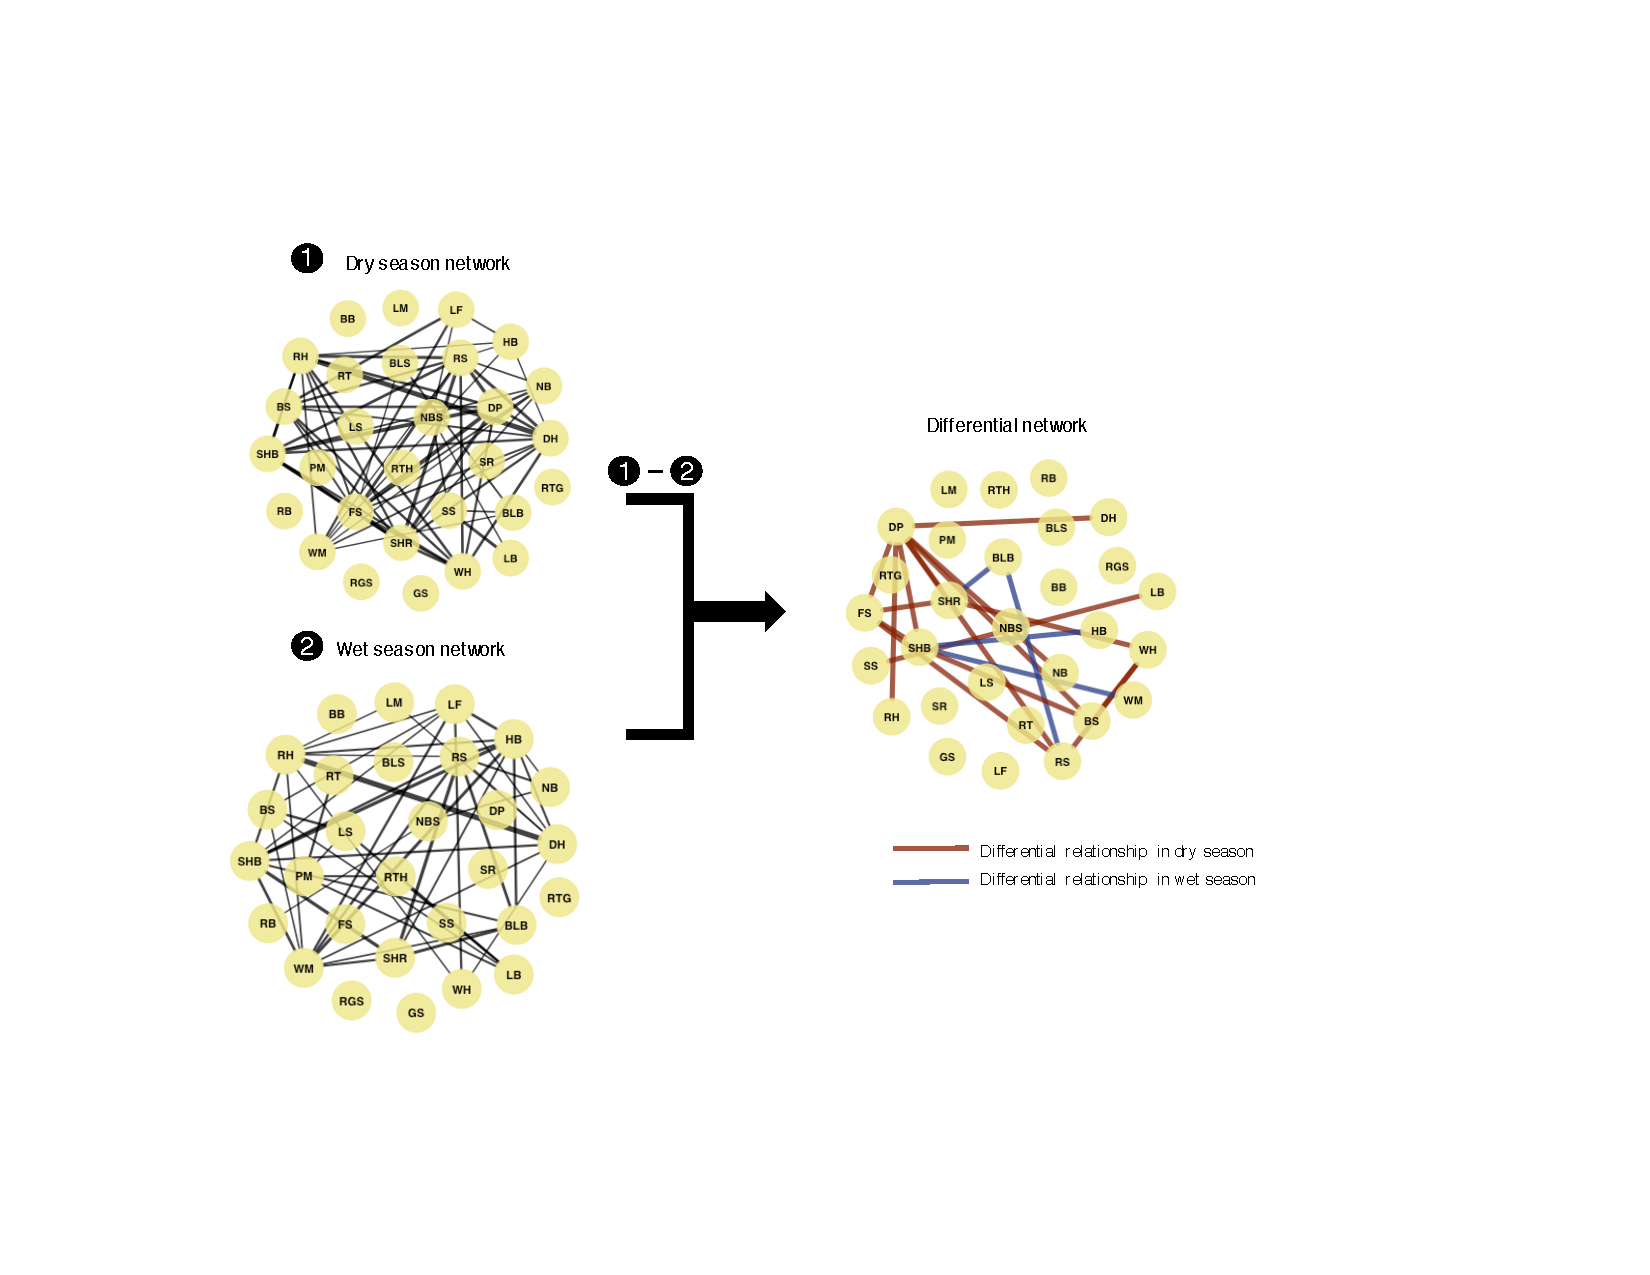
\includegraphics[width = 0.8\textwidth]{figures/pipeline3.pdf}
\caption{Schematic showing principle of differential analysis in seasons. Co-occurrence networks are measured in each of two seasons (left) resulting in interactions (black). Dry season is subtracted from wet season to create a differential co-occurrence network (right), in which the significant differential interactions are those that positive (red) or negative (blue) in score after the shift in conditions, which means differential in dry, and wet season, respectively.}
\label{fig:pipeline3}
\end{figure} 

\textbf{Difference of co-occurrence network of rice injuries at different yield levels}

Consider any two injuries $x$ and $y$ in the survey data, let $r_{xy}^L$ and $r_{xy}^H$ be the Spearman’s correlation coefficient calculated separately over the samples in $L$ and $H$ yield level, respectively. I constructed differential co-occurrence networks that are specified by adjacency matrix $A^{diff}$ = $(A_{xy}^{diff})$ where the entry $A_{xy}^{diff}$ quantified by following:   

\begin{equation}
A_{xy}^{diff} = \left\{\begin{matrix} 1 & \text{when } r_{xy}^L > r_{xy}^H \text{ at } P_{z_{xy}} \text{-value} < 0.05  \\  0 & \text{otherwise}                             
\end{matrix}\right.
\end{equation}

For  this differential co-occurrence network,$A_{xy}^{diff}$ equals 1 depending on whether any injury pairs show significantly higher co-occurrence level in low yield level than high yield state, and if it equal 0, meaning that co-occurrence level of injury pairs were not or lower different in low yield level state. \ref{fig:pipeline4} illustrated the differential co-occurrence network at different seasons.

\begin{figure}
\centering
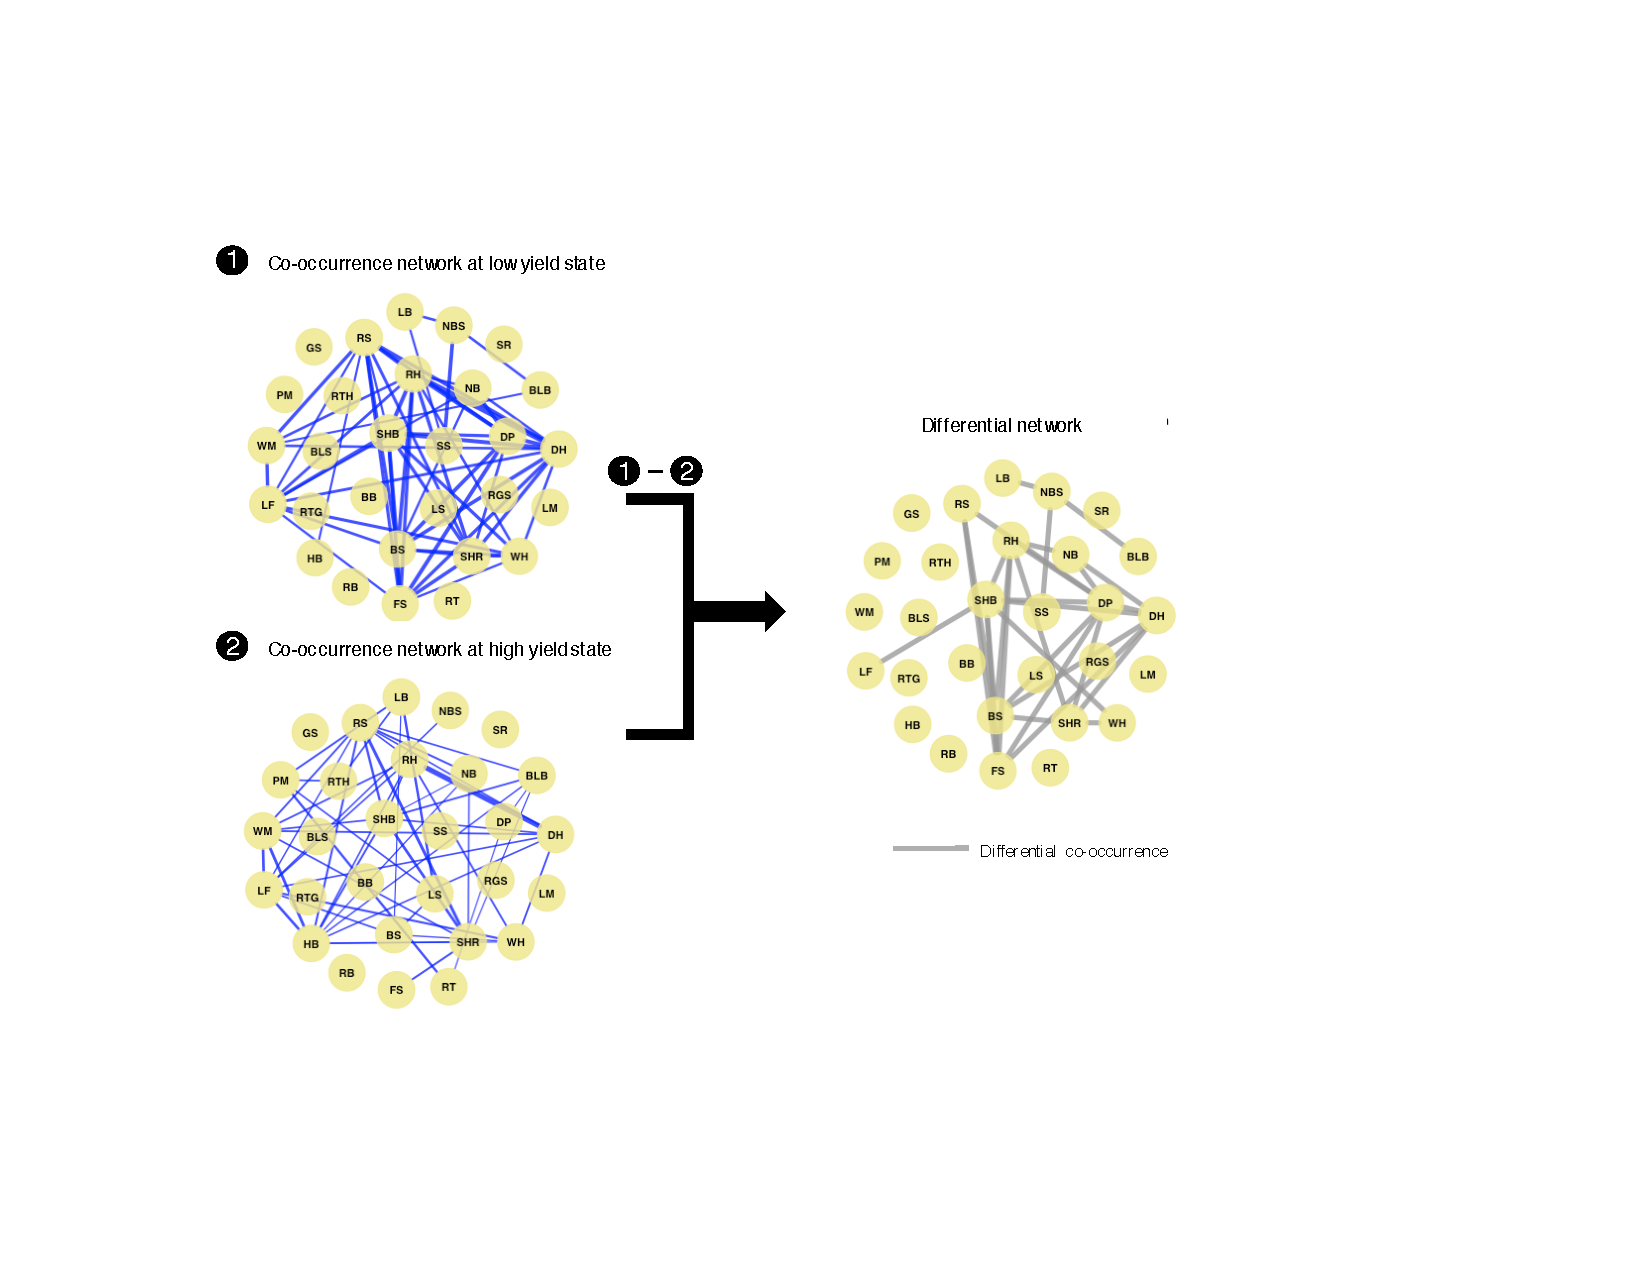
\includegraphics[width = 0.8\textwidth]{figures/pipeline4.pdf}
\caption{Schematic showing differential analysis at different yield levels. Co-occurrence networks are measured in each of two different yield levels (left) resulting in interactions (blue). The network at low yield level network is subtracted from high yield level to create a differential co-occurrence network (right), in which the significant differential interactions are those that positive in score after the shift from low to high yield state.}
\label{fig:pipeline4}
\end{figure} 

\textbf{Topological properties}
To investigate the structural properties of differential networks, I calculated topological features for each node in the network with the \textbf{igraph} package. This feature set included node degree, clustering coefficient, and betweenness. 


\section{Results}

\subsection{Construction of differential co-occurrence networks of rice injuries at different seasons}

I determined which co-occurrence patterns of rice injuires of survey data were differentially expressed between dry and wet season. The resulted networks are showed in \ref{fig:difseasonCP}) to Figure.\ref{fig:difseasonWJ}). Differential co-occurrence network (DCON) in seasons at CP (Figure. \ref{fig:difseasonCP}) reveals SHB, RS, SHB showing significantly different co-occurrence level in both dry and wet season. DCON in season at OD \ref{fig:difseasonOD}
reveals LB different both in dry and wet season. DCON in season at RR \ref{fig:difseasonRR}  reveals that DP, BS, RTH, LF. DCON in season at WJ (Figure.\ref{fig:difseasonWJ} revealed that  BS, NBS, SHB BLS. \ref{fig:difseasonTM}

\begin{figure}
\centering
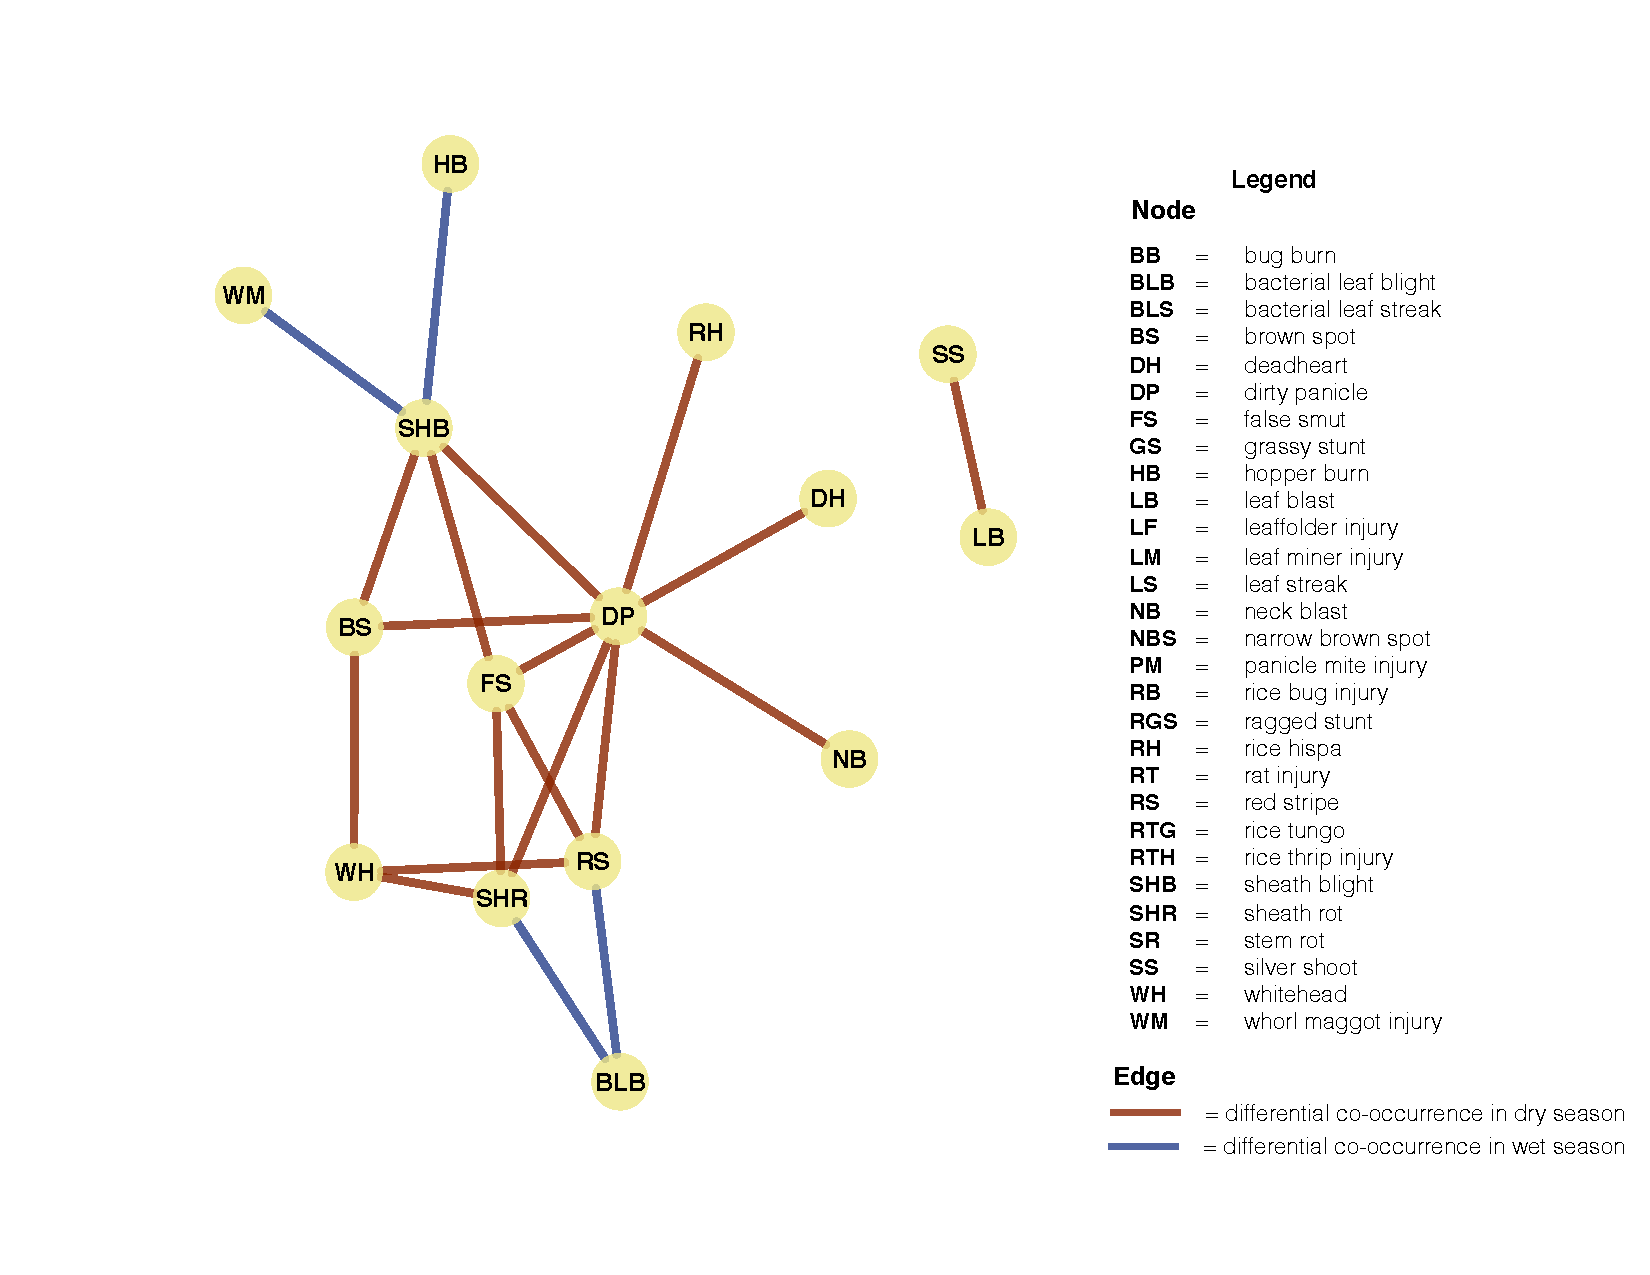
\includegraphics[width = 1\textwidth]{figures/difseasonCP.pdf}
\caption{Differential co-occurrence network of rice injuries in different seasons at Central Plain, Thailand}
\label{fig:difseasonCP}
\end{figure} 

\begin{figure}
\centering
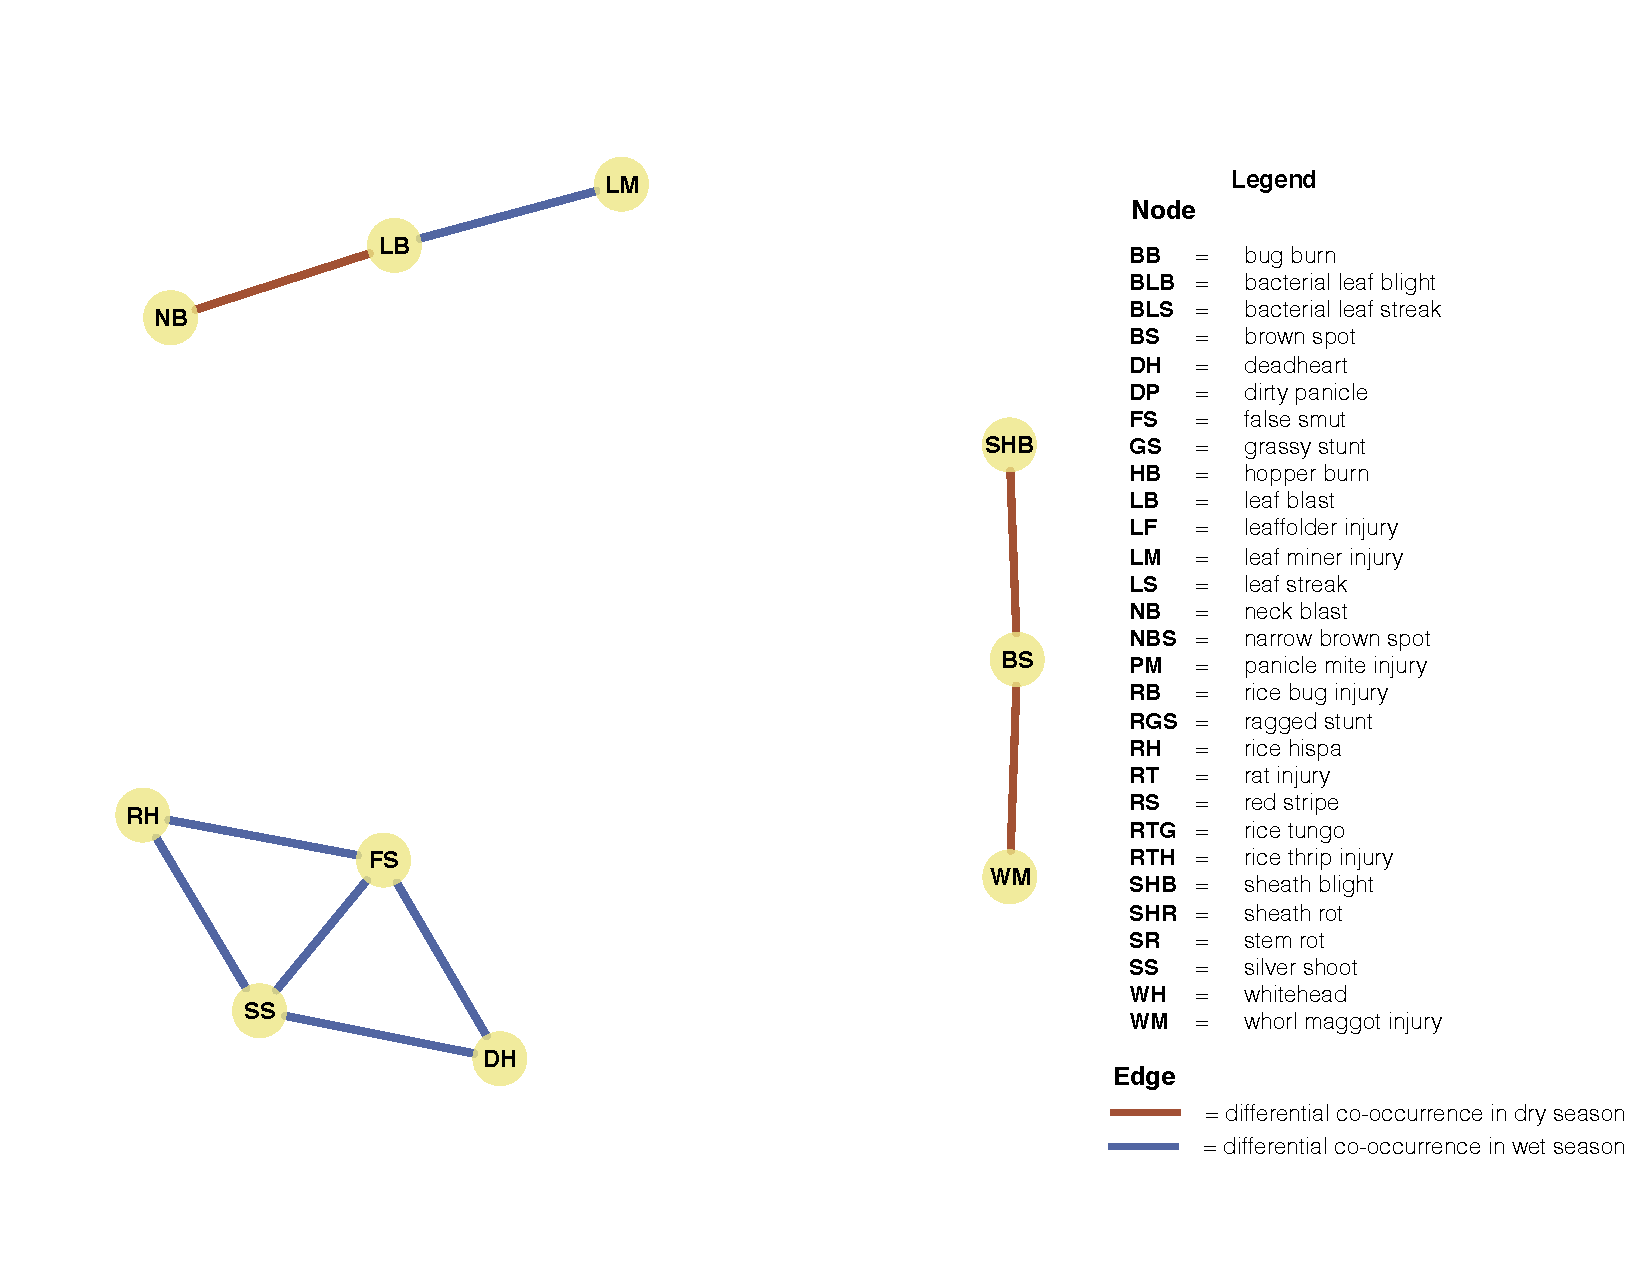
\includegraphics[width = 1\textwidth]{figures/difseasonOR.pdf}
\caption{Differential co-occurrence network of rice injuries in different seasons at Odisha, India }
\label{fig:difseasonOR}
\end{figure}


\begin{figure}
\centering
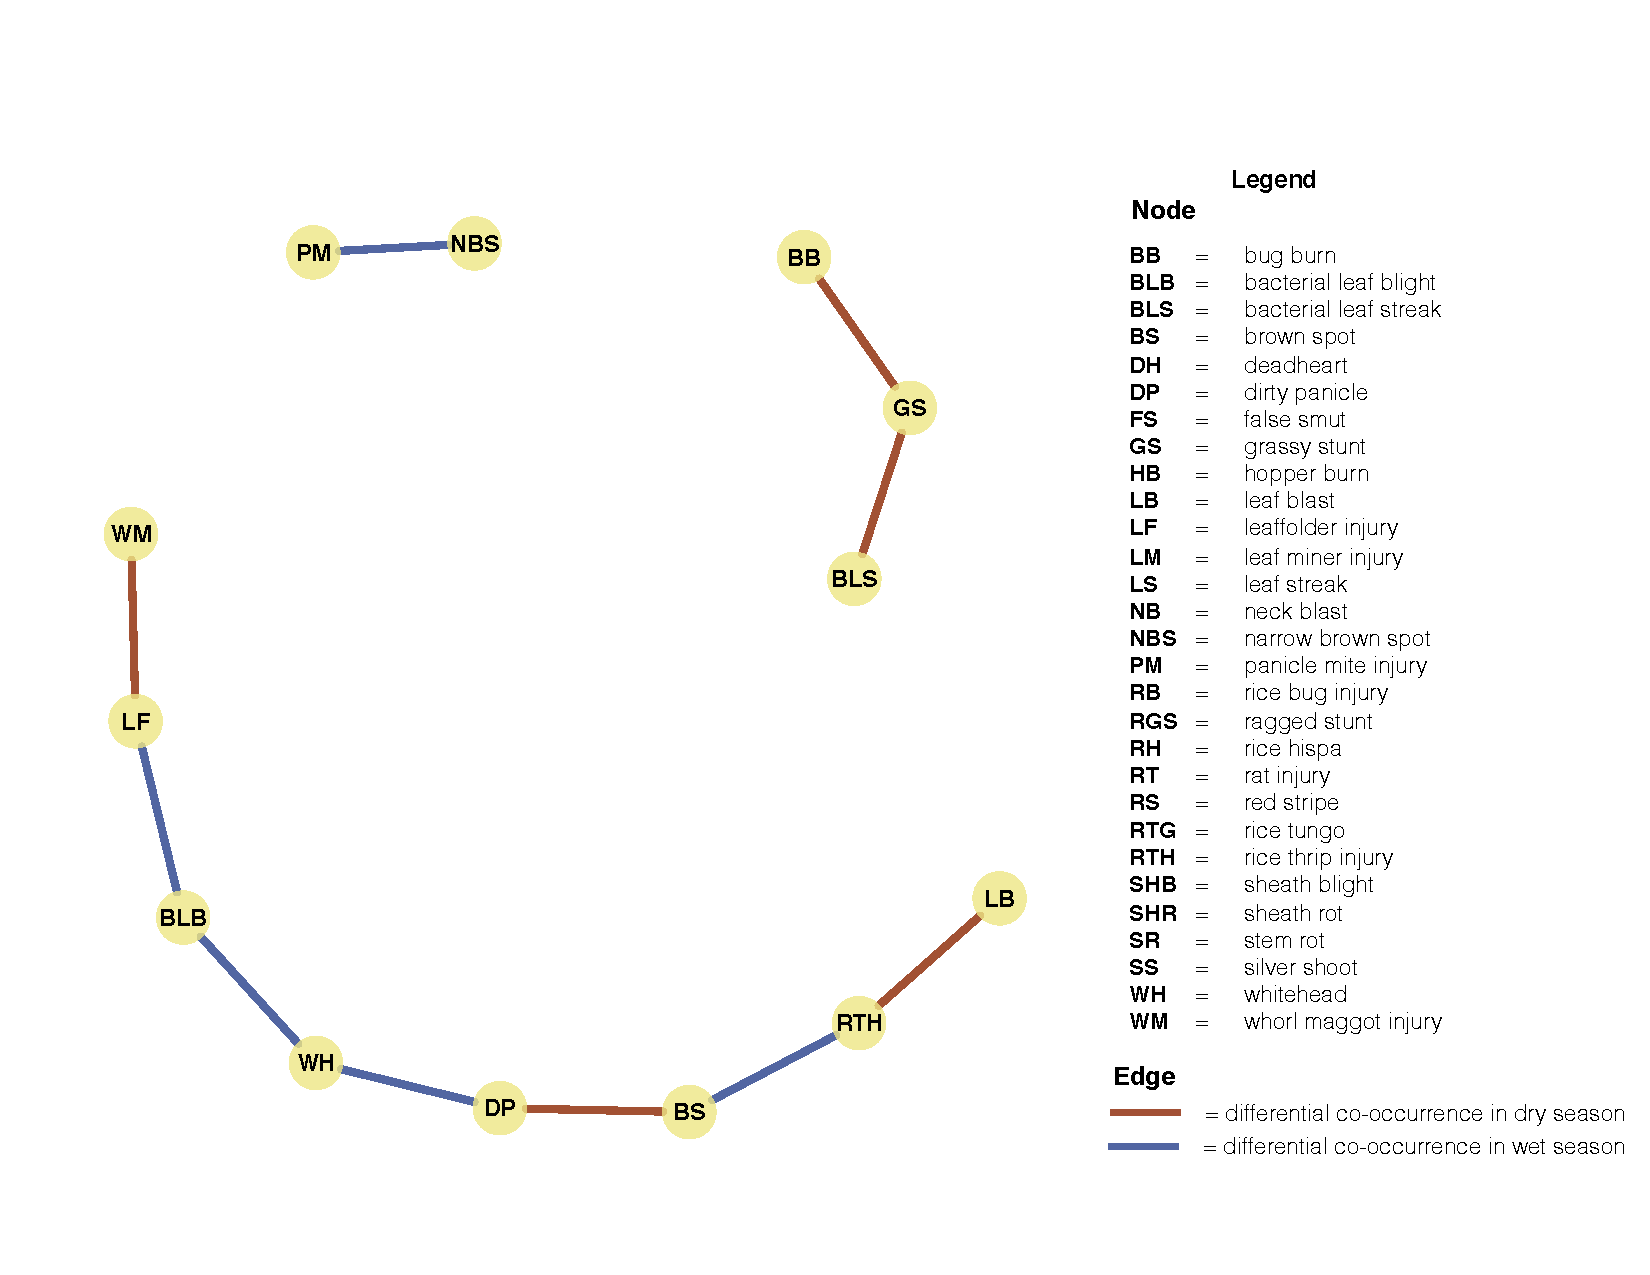
\includegraphics[width = 1\textwidth]{figures/difseasonRR.pdf}
\caption{Differential co-occurrence network of rice injuries in different seasons at Red River Delta, Vietnam}
\label{fig:difseasonRR}
\end{figure}


\begin{figure}
\centering
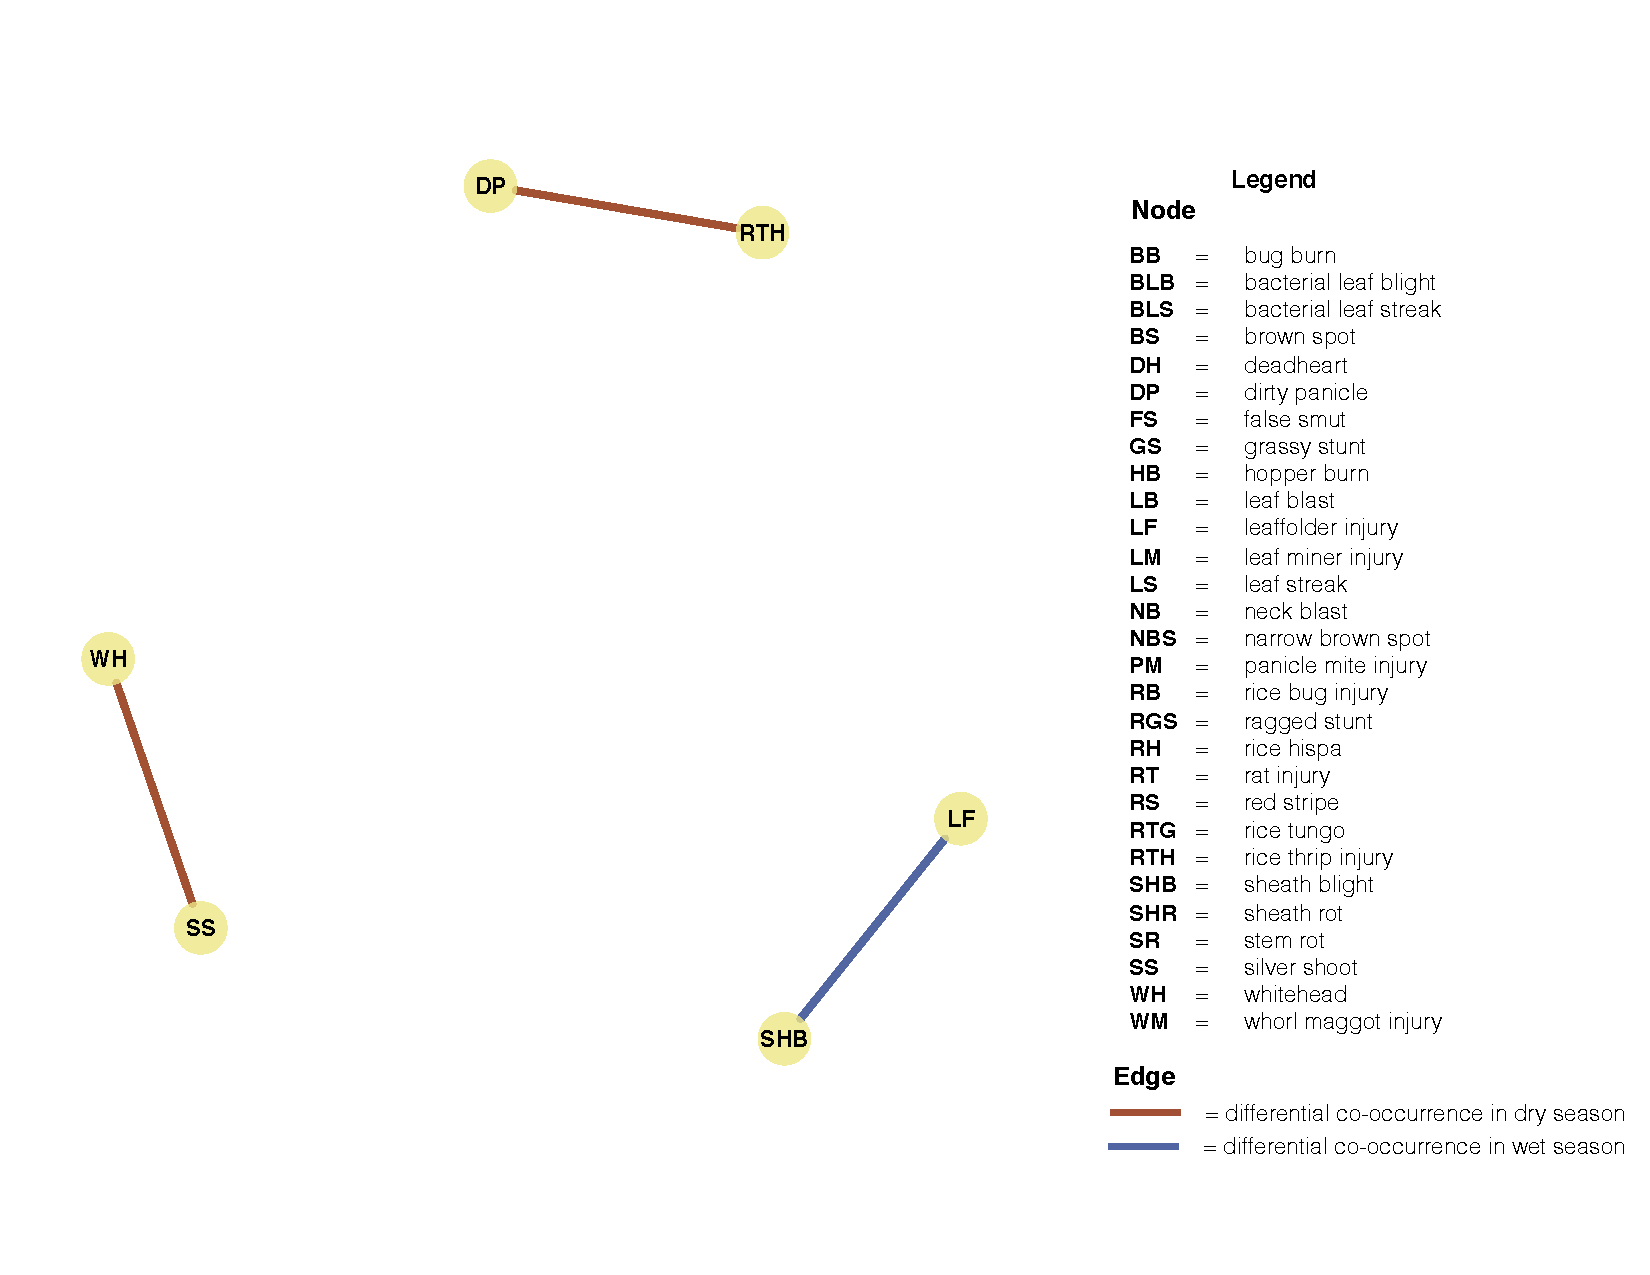
\includegraphics[width = 1\textwidth]{figures/difseasonTM.pdf}
\caption{Differential co-occurrence network of rice injuries in different seasons at Tamil Nadu, India}
\label{fig:difseasonTM}
\end{figure}


\begin{figure}
\centering
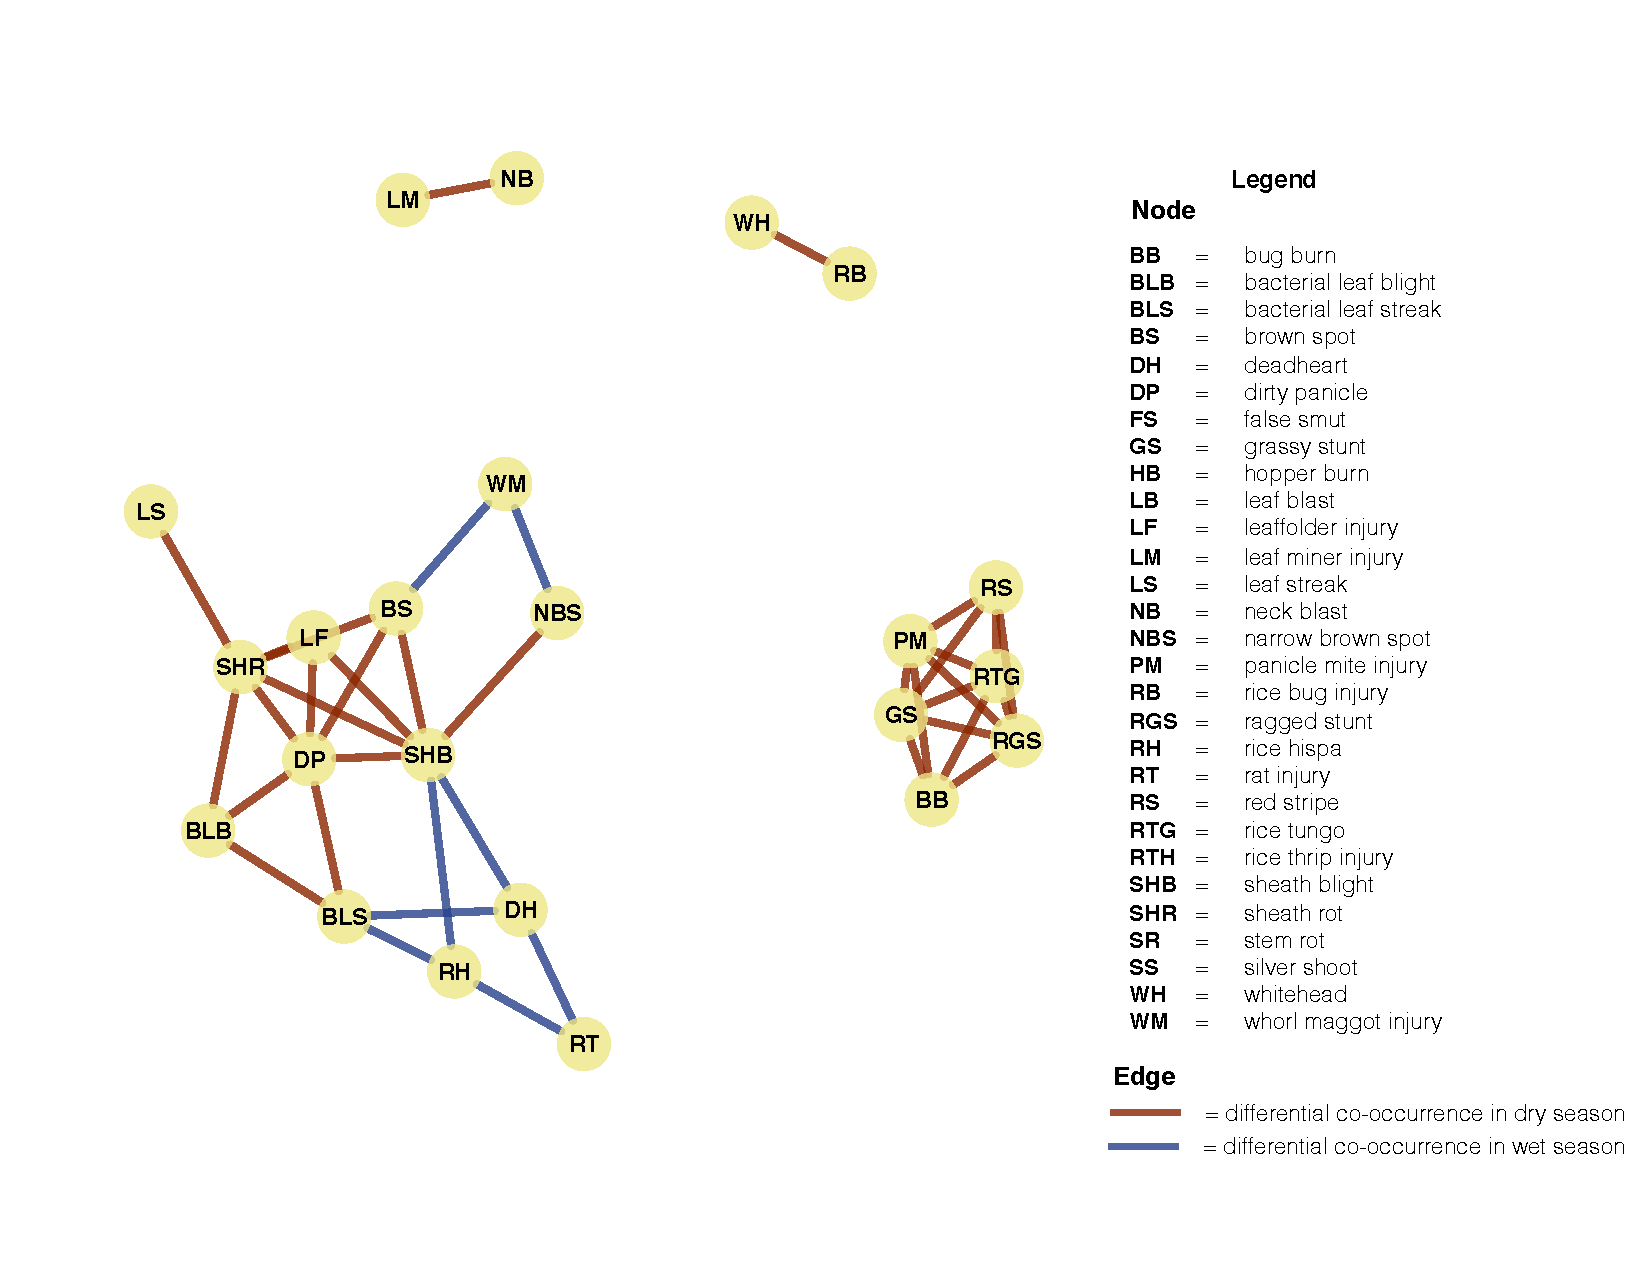
\includegraphics[width = 1\textwidth]{figures/difseasonWJ.pdf}
\caption{Differential co-occurrence network of rice injuries in different seasons at West Java, Indonesia}
\label{fig:difseasonWJ}
\end{figure}

%================================
\subsection{Construction of differential co-occurrence networks of rice injuries at yield level}

In this study, three successive yield classes were defined, in order to enable a better description of actual yield, from low (< 4 ton/ha), medium (4 – 6 ton/ha) ,  high (> 6 ton/ha) yield levels. Figure \ref{fig: yield_level_bar} shows the number of farmers’ fields surveyed classified in each season, and production environment.

\citet{Berry_2014_Deciphering} recommended that a co-occurrence network will be more reliable, it should be produced using a minimum of 25 samples or observations. From figure \ref{fig: yield_level_bar}, to be able compare the networks at different yield levels, I chose the data set, which are medium and high yield level of CP, low and medium yield level of TM, medium and high yield level at RR, low and medium yield level of TM, and medium and high yield level of WJ. 

In this study, an differential co-occurrence network (DCON) in yield depicts the associations of injury pairs presenting in lower yield state but absent in higher yield state (Figures. \ref{fig:difyieldCP}, \ref{fig:difyieldOD}, \ref{fig:difyieldRR}, \ref{fig:difyieldTM}, \ref{fig:difyieldWJ}).  DCON

\begin{figure}
    \centering
        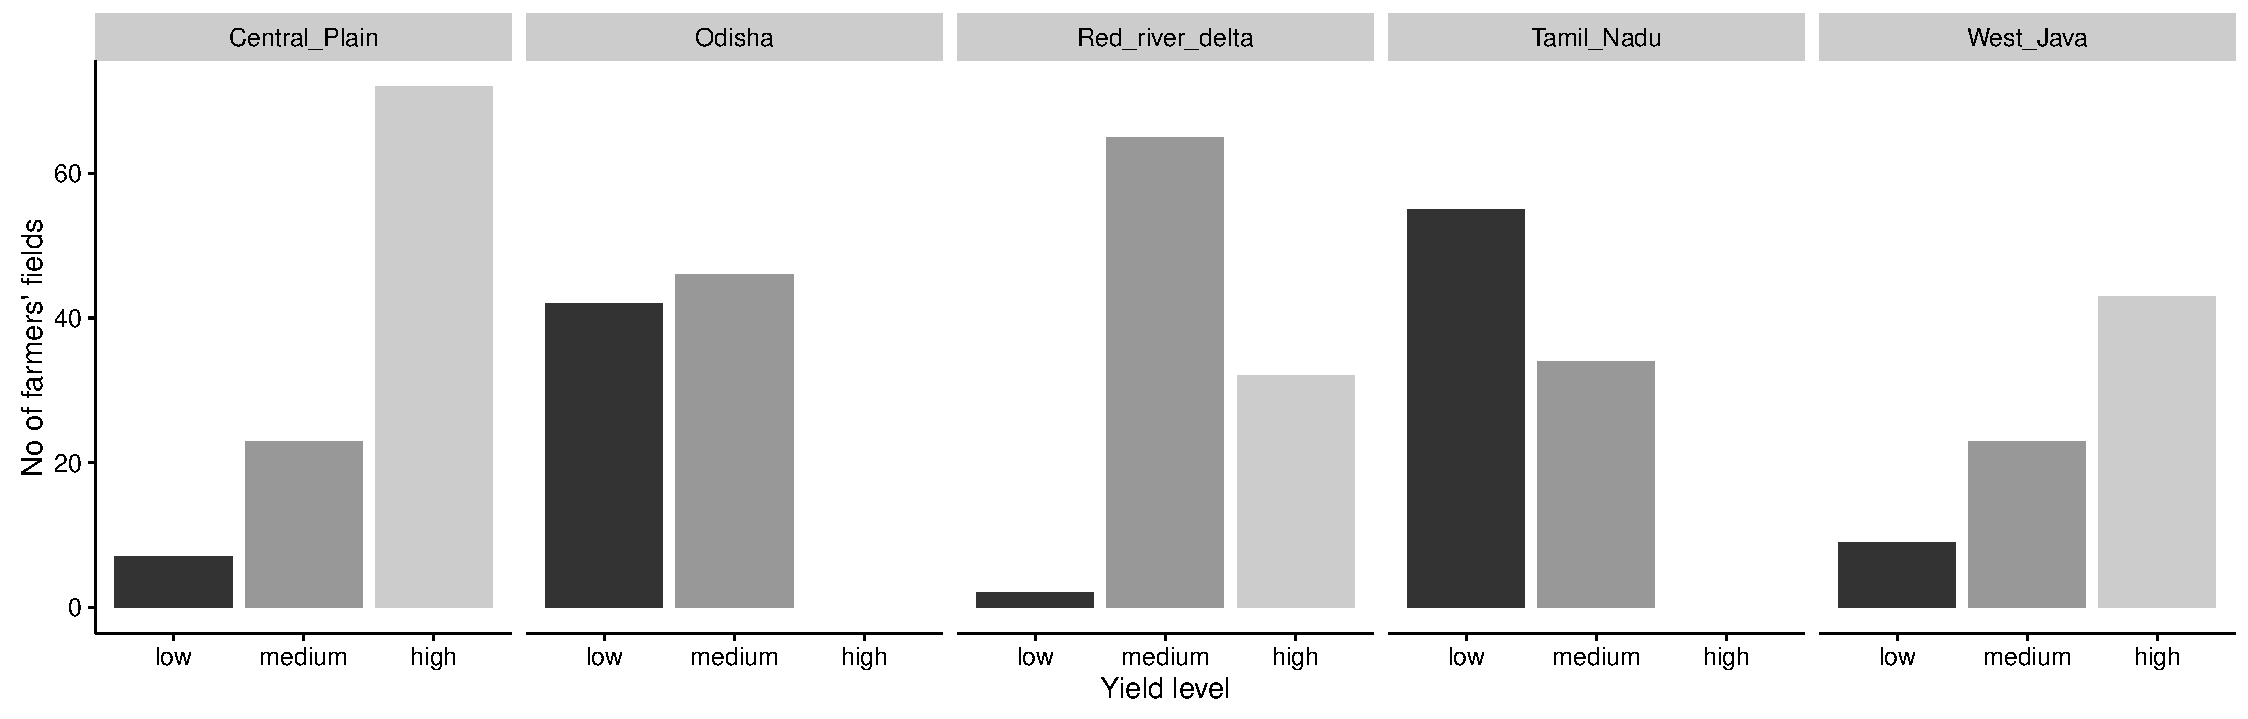
\includegraphics[width = 1\textwidth]{figures/yield_level_bar.pdf}
        \caption{.}
        \label{fig: yield_level_bar}
\end{figure}

\begin{figure}
    \centering
    \begin{subfigure}[b]{1\textwidth}
        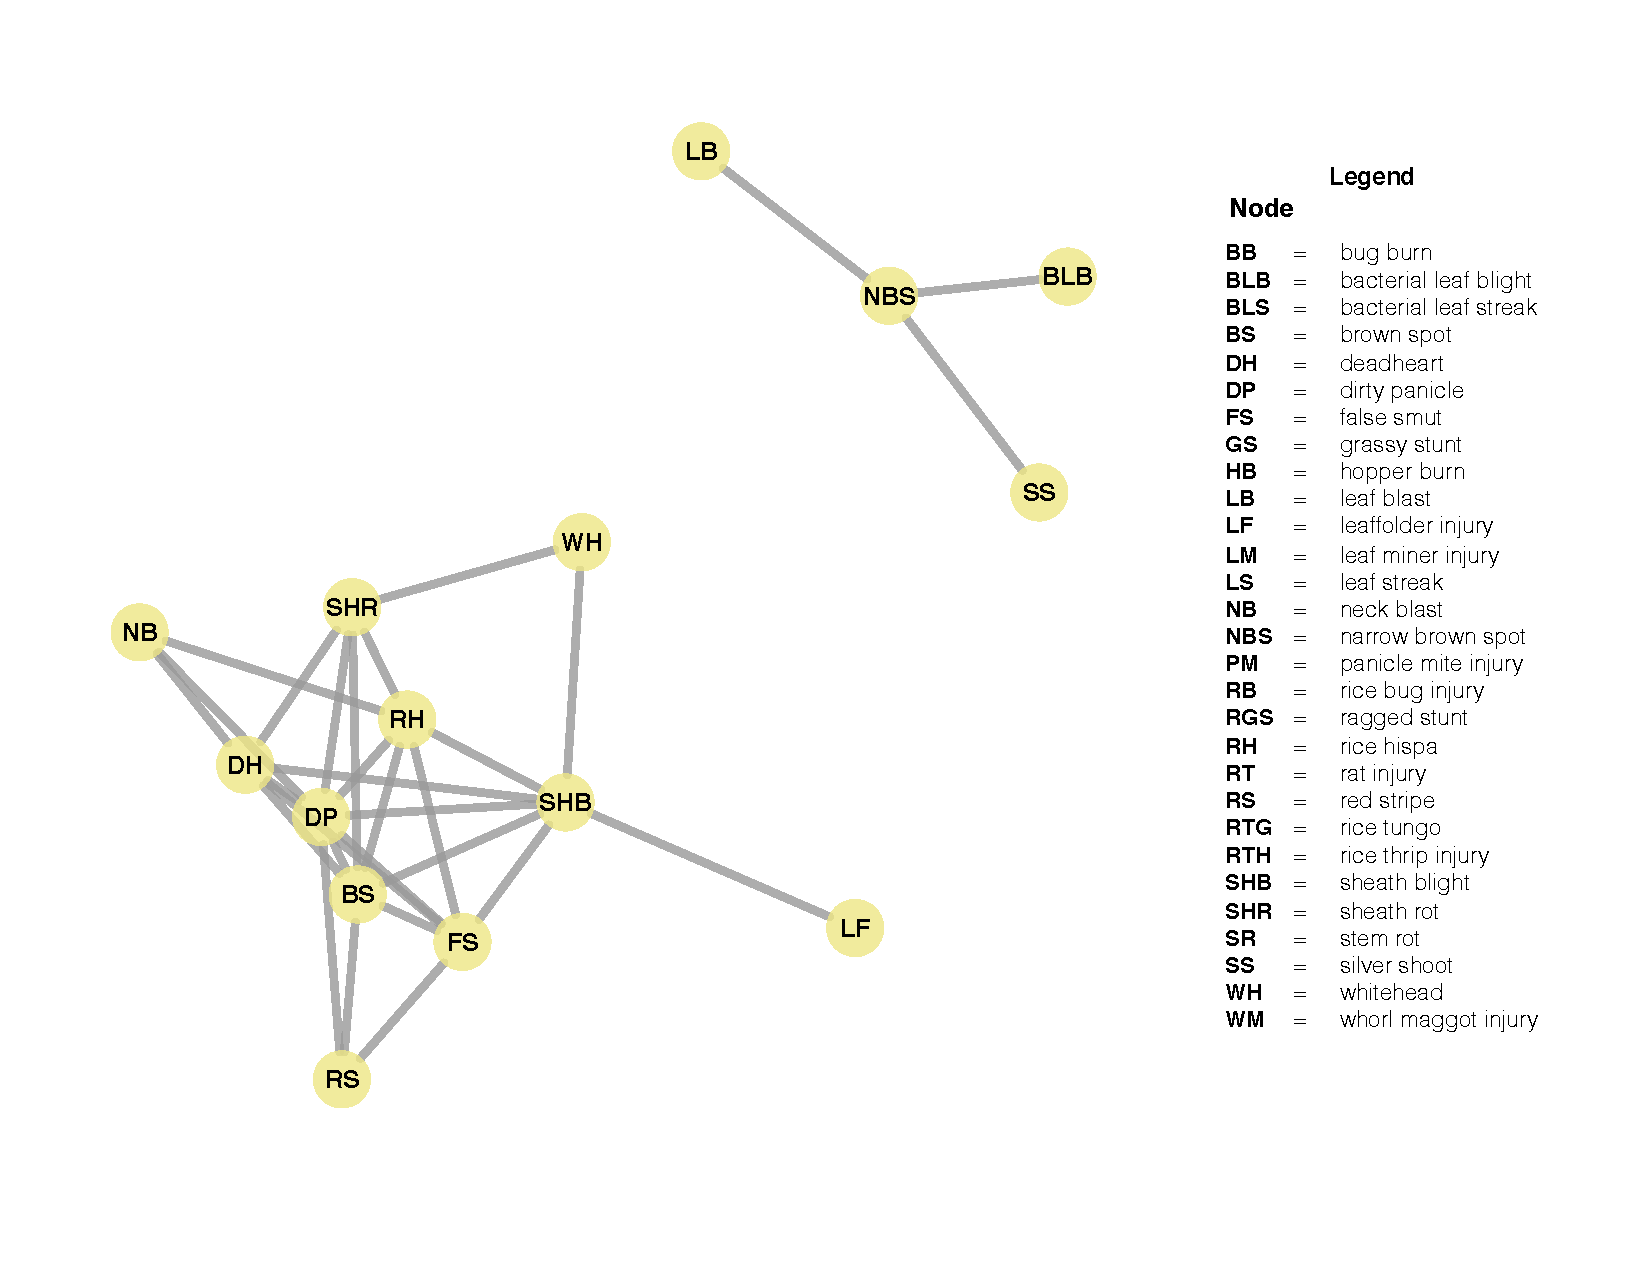
\includegraphics[width = 1\textwidth]{figures/difyieldCP.pdf}
        \caption{Differential co-occurrence network of rice injuries in different yield levels at Central Plain, Thailand. The layout of the network graph is based on the Fruchterman-Reingold algorithm, which places nodes with stronger or more connections closer to each other.}
        \label{fig:networkCP_ds}
    \end{subfigure}
    \begin{subfigure}[b]{1\textwidth}
        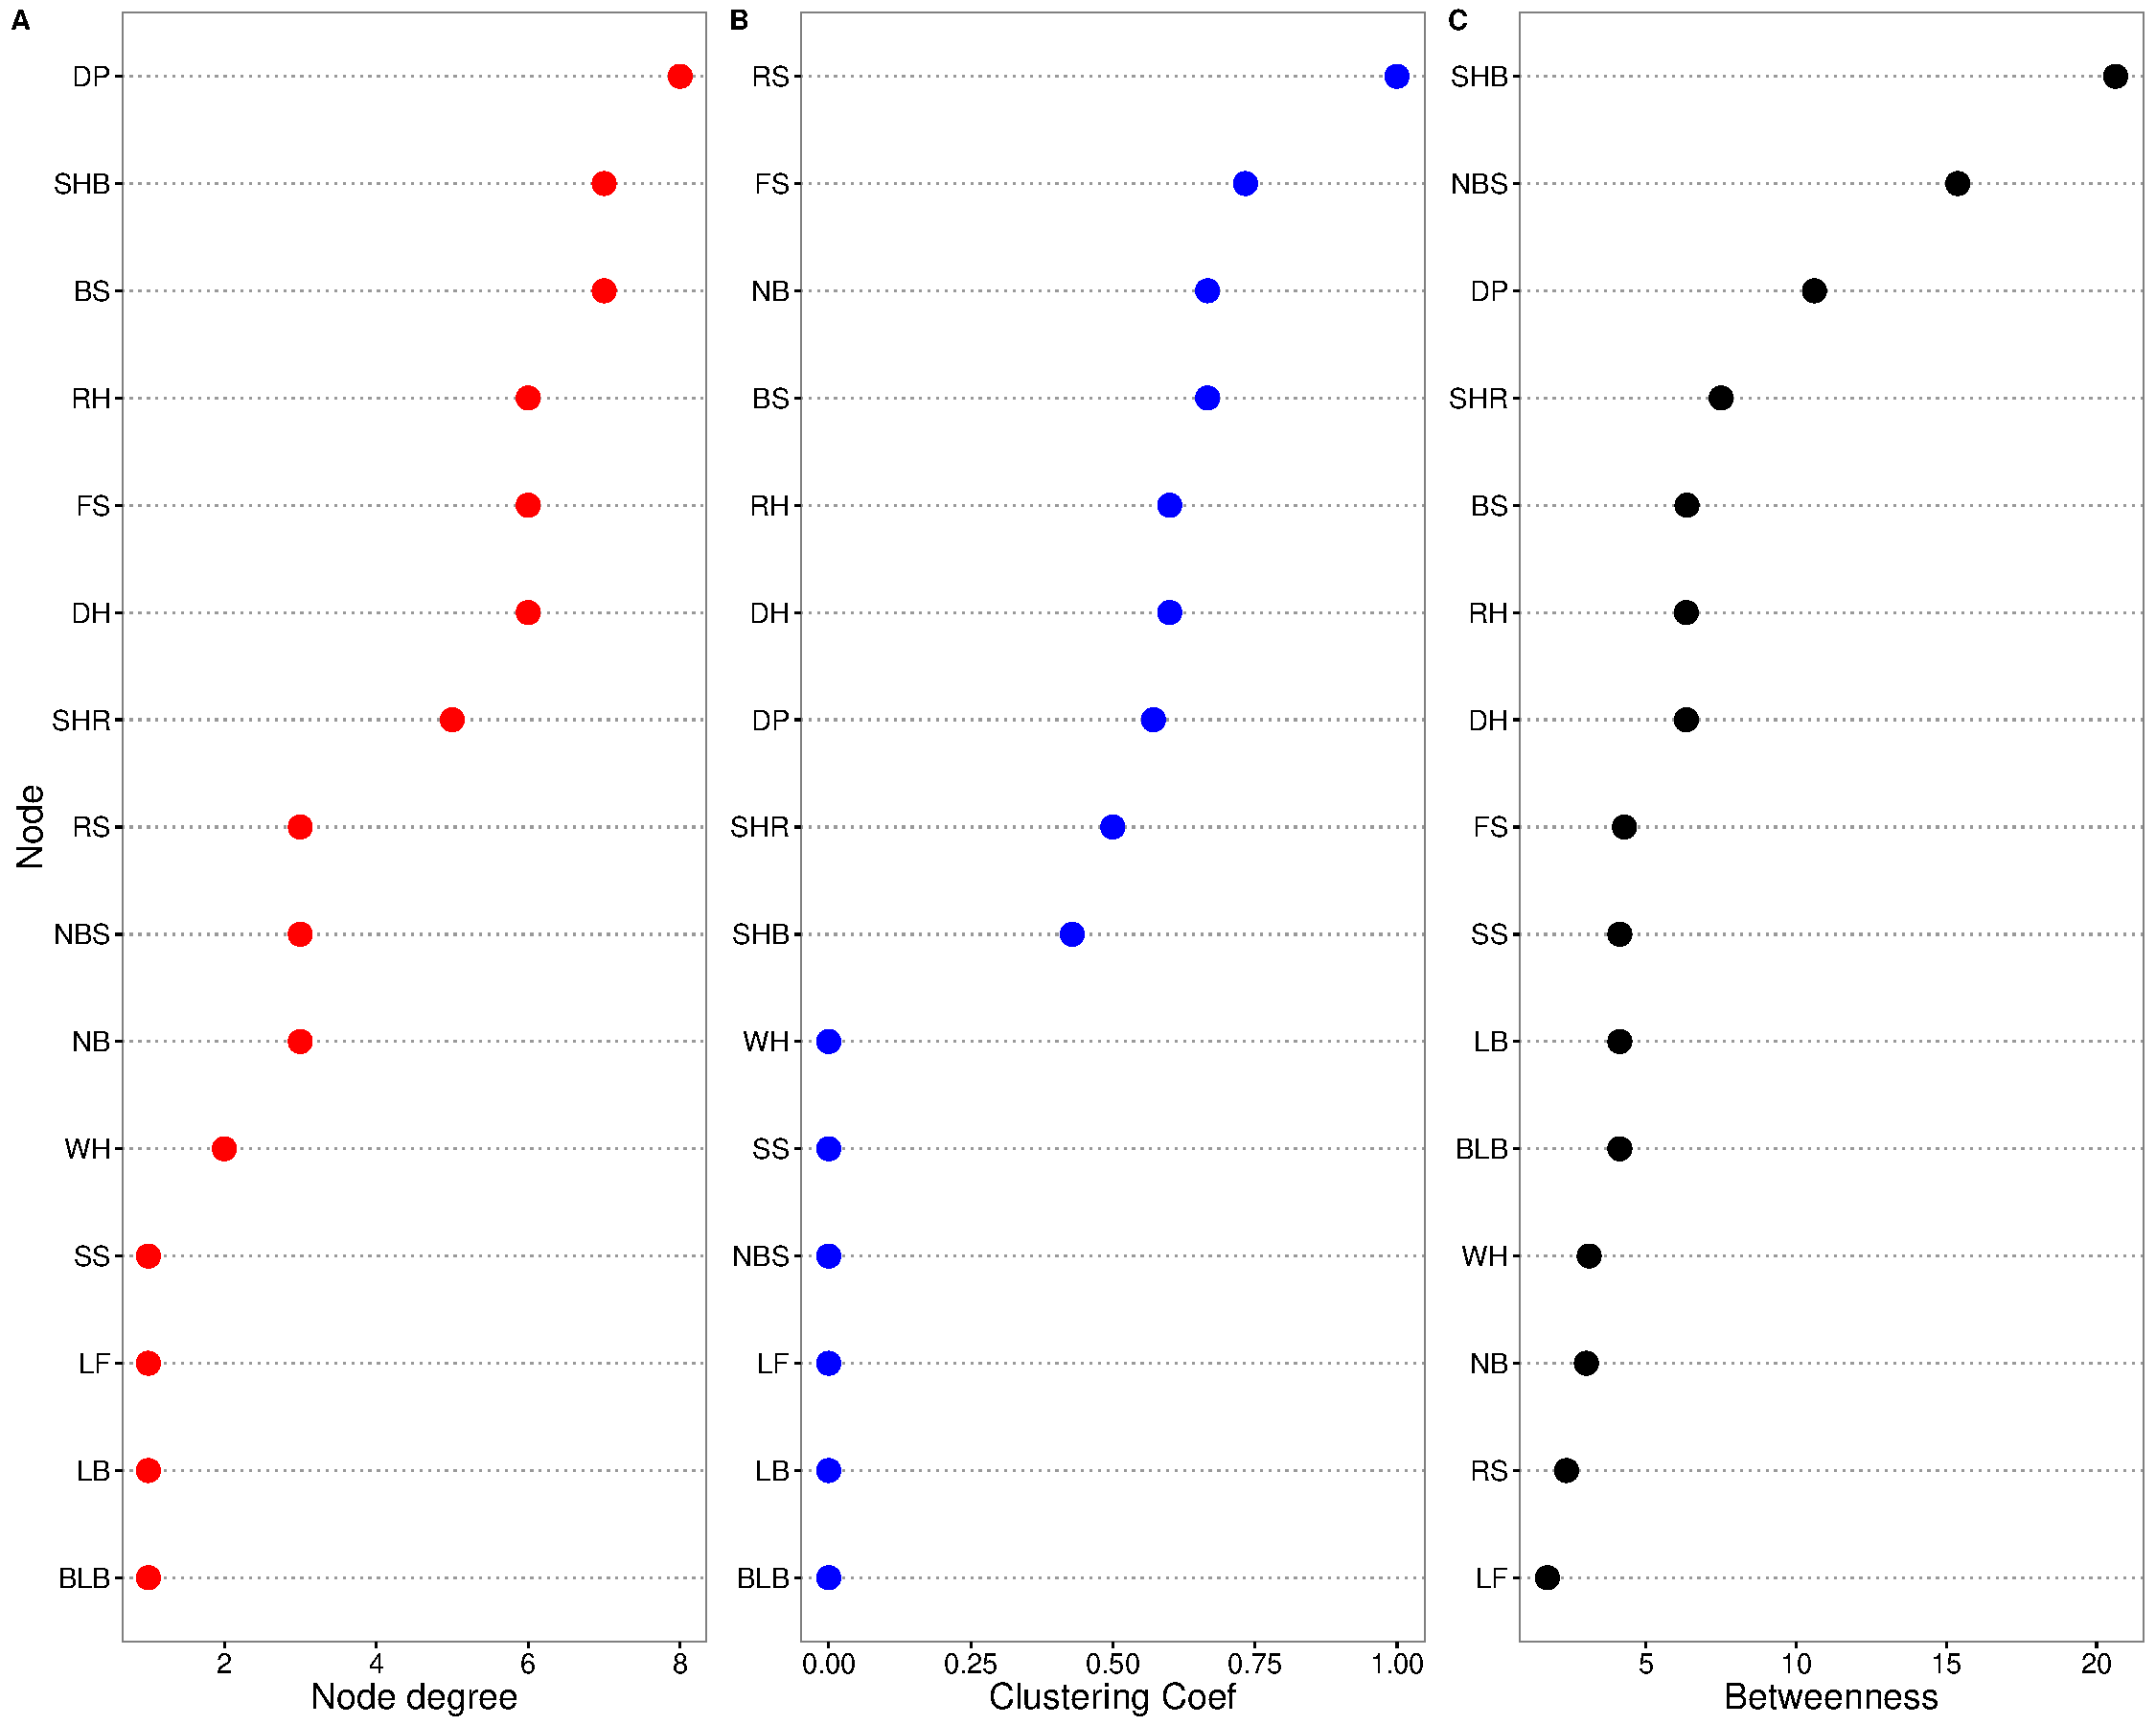
\includegraphics[width = 1\textwidth]{figures/yield_dif_nodepropCentral_Plain.pdf}
        \caption{Three centrality measures of the nodes in co-occurrence network of rice injuries in dry season at Central Plain. A: node degree, B:clustering coefficient, and C:Betweenness.}
        \label{fig:nodepropCP_ds}
    \end{subfigure}
    \caption{Rice injuries in dry season in Central Plain, Thailand}
    \label{fig:CP_ds}
\end{figure}
 
\begin{figure}
    \centering
    \begin{subfigure}[b]{1\textwidth}
        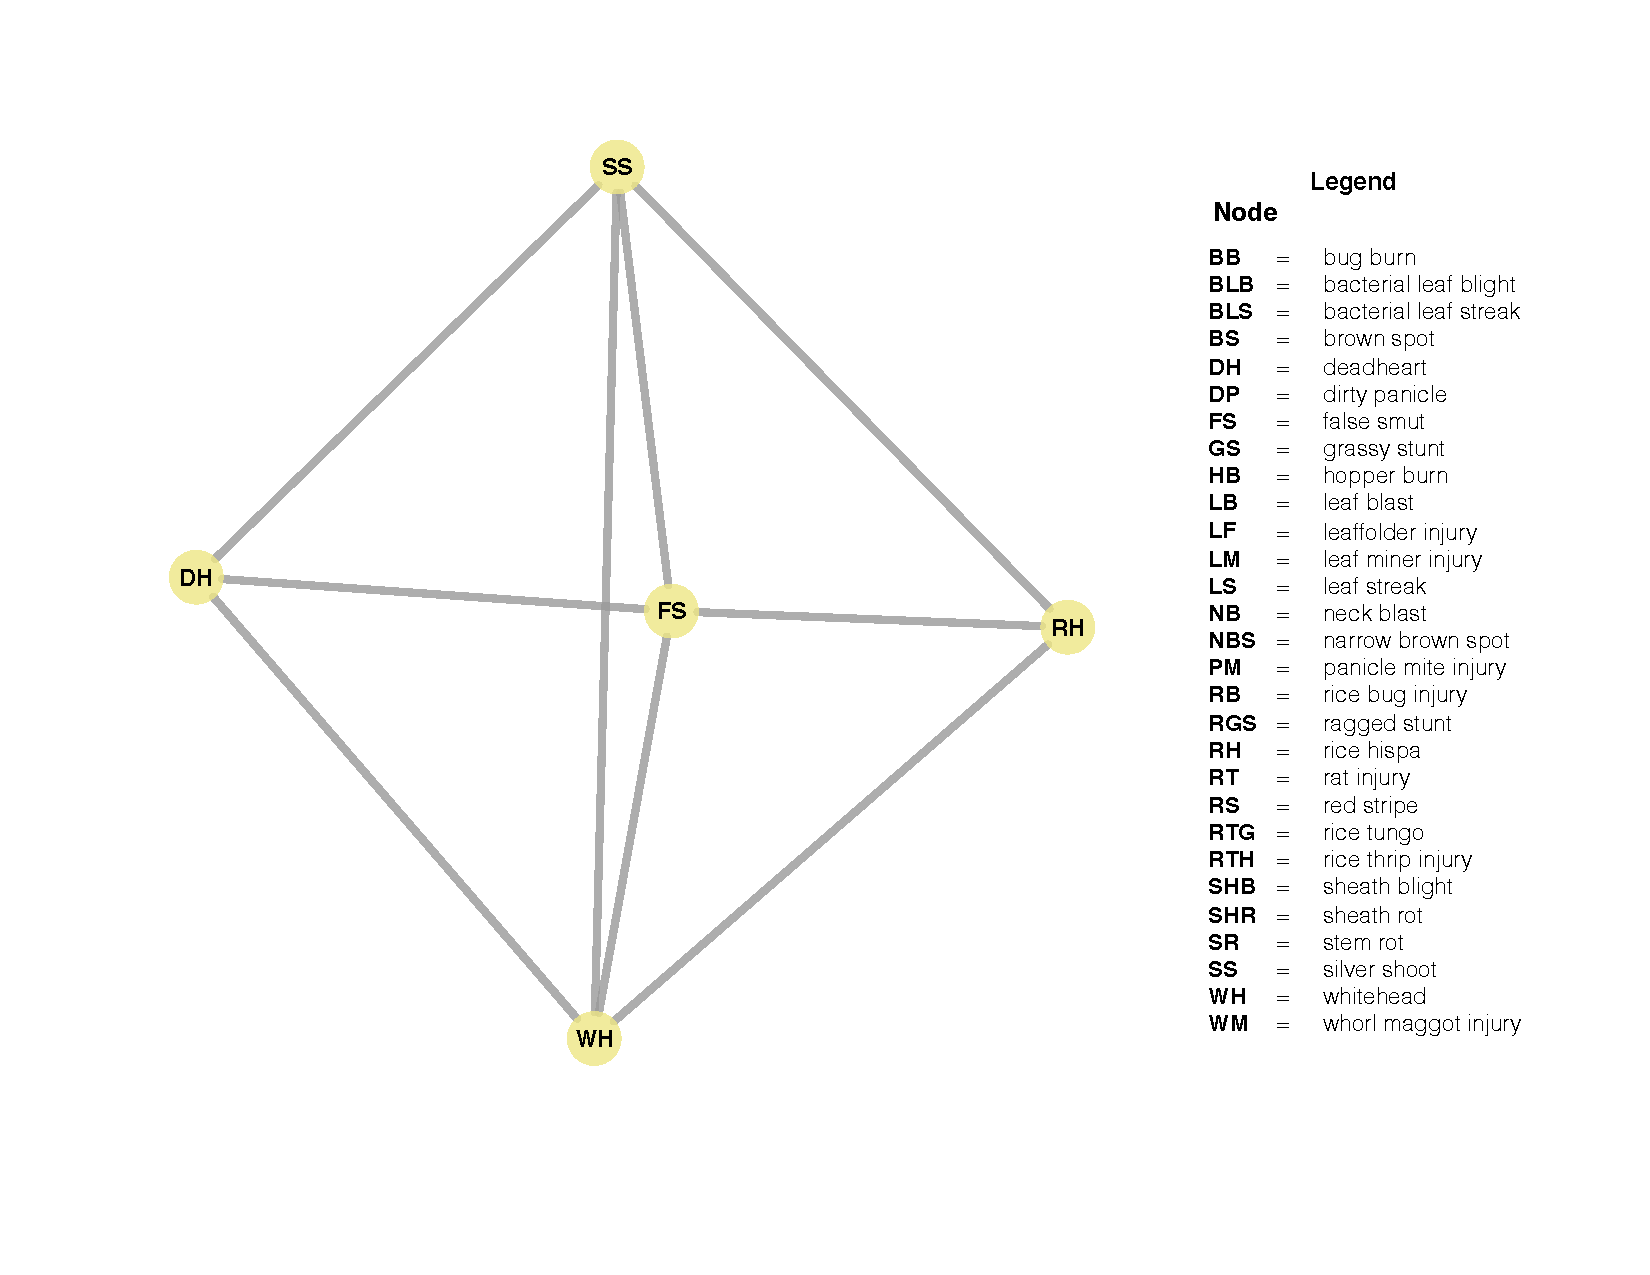
\includegraphics[width = 1\textwidth]{figures/difyieldOD.pdf}
        \caption{Differential co-occurrence network of rice injuries in different yield levels at Central Plain, Thailand. The layout of the network graph is based on the Fruchterman-Reingold algorithm, which places nodes with stronger or more connections closer to each other.}
        \label{fig:difyieldOD}
    \end{subfigure}
    \begin{subfigure}[b]{1\textwidth}
        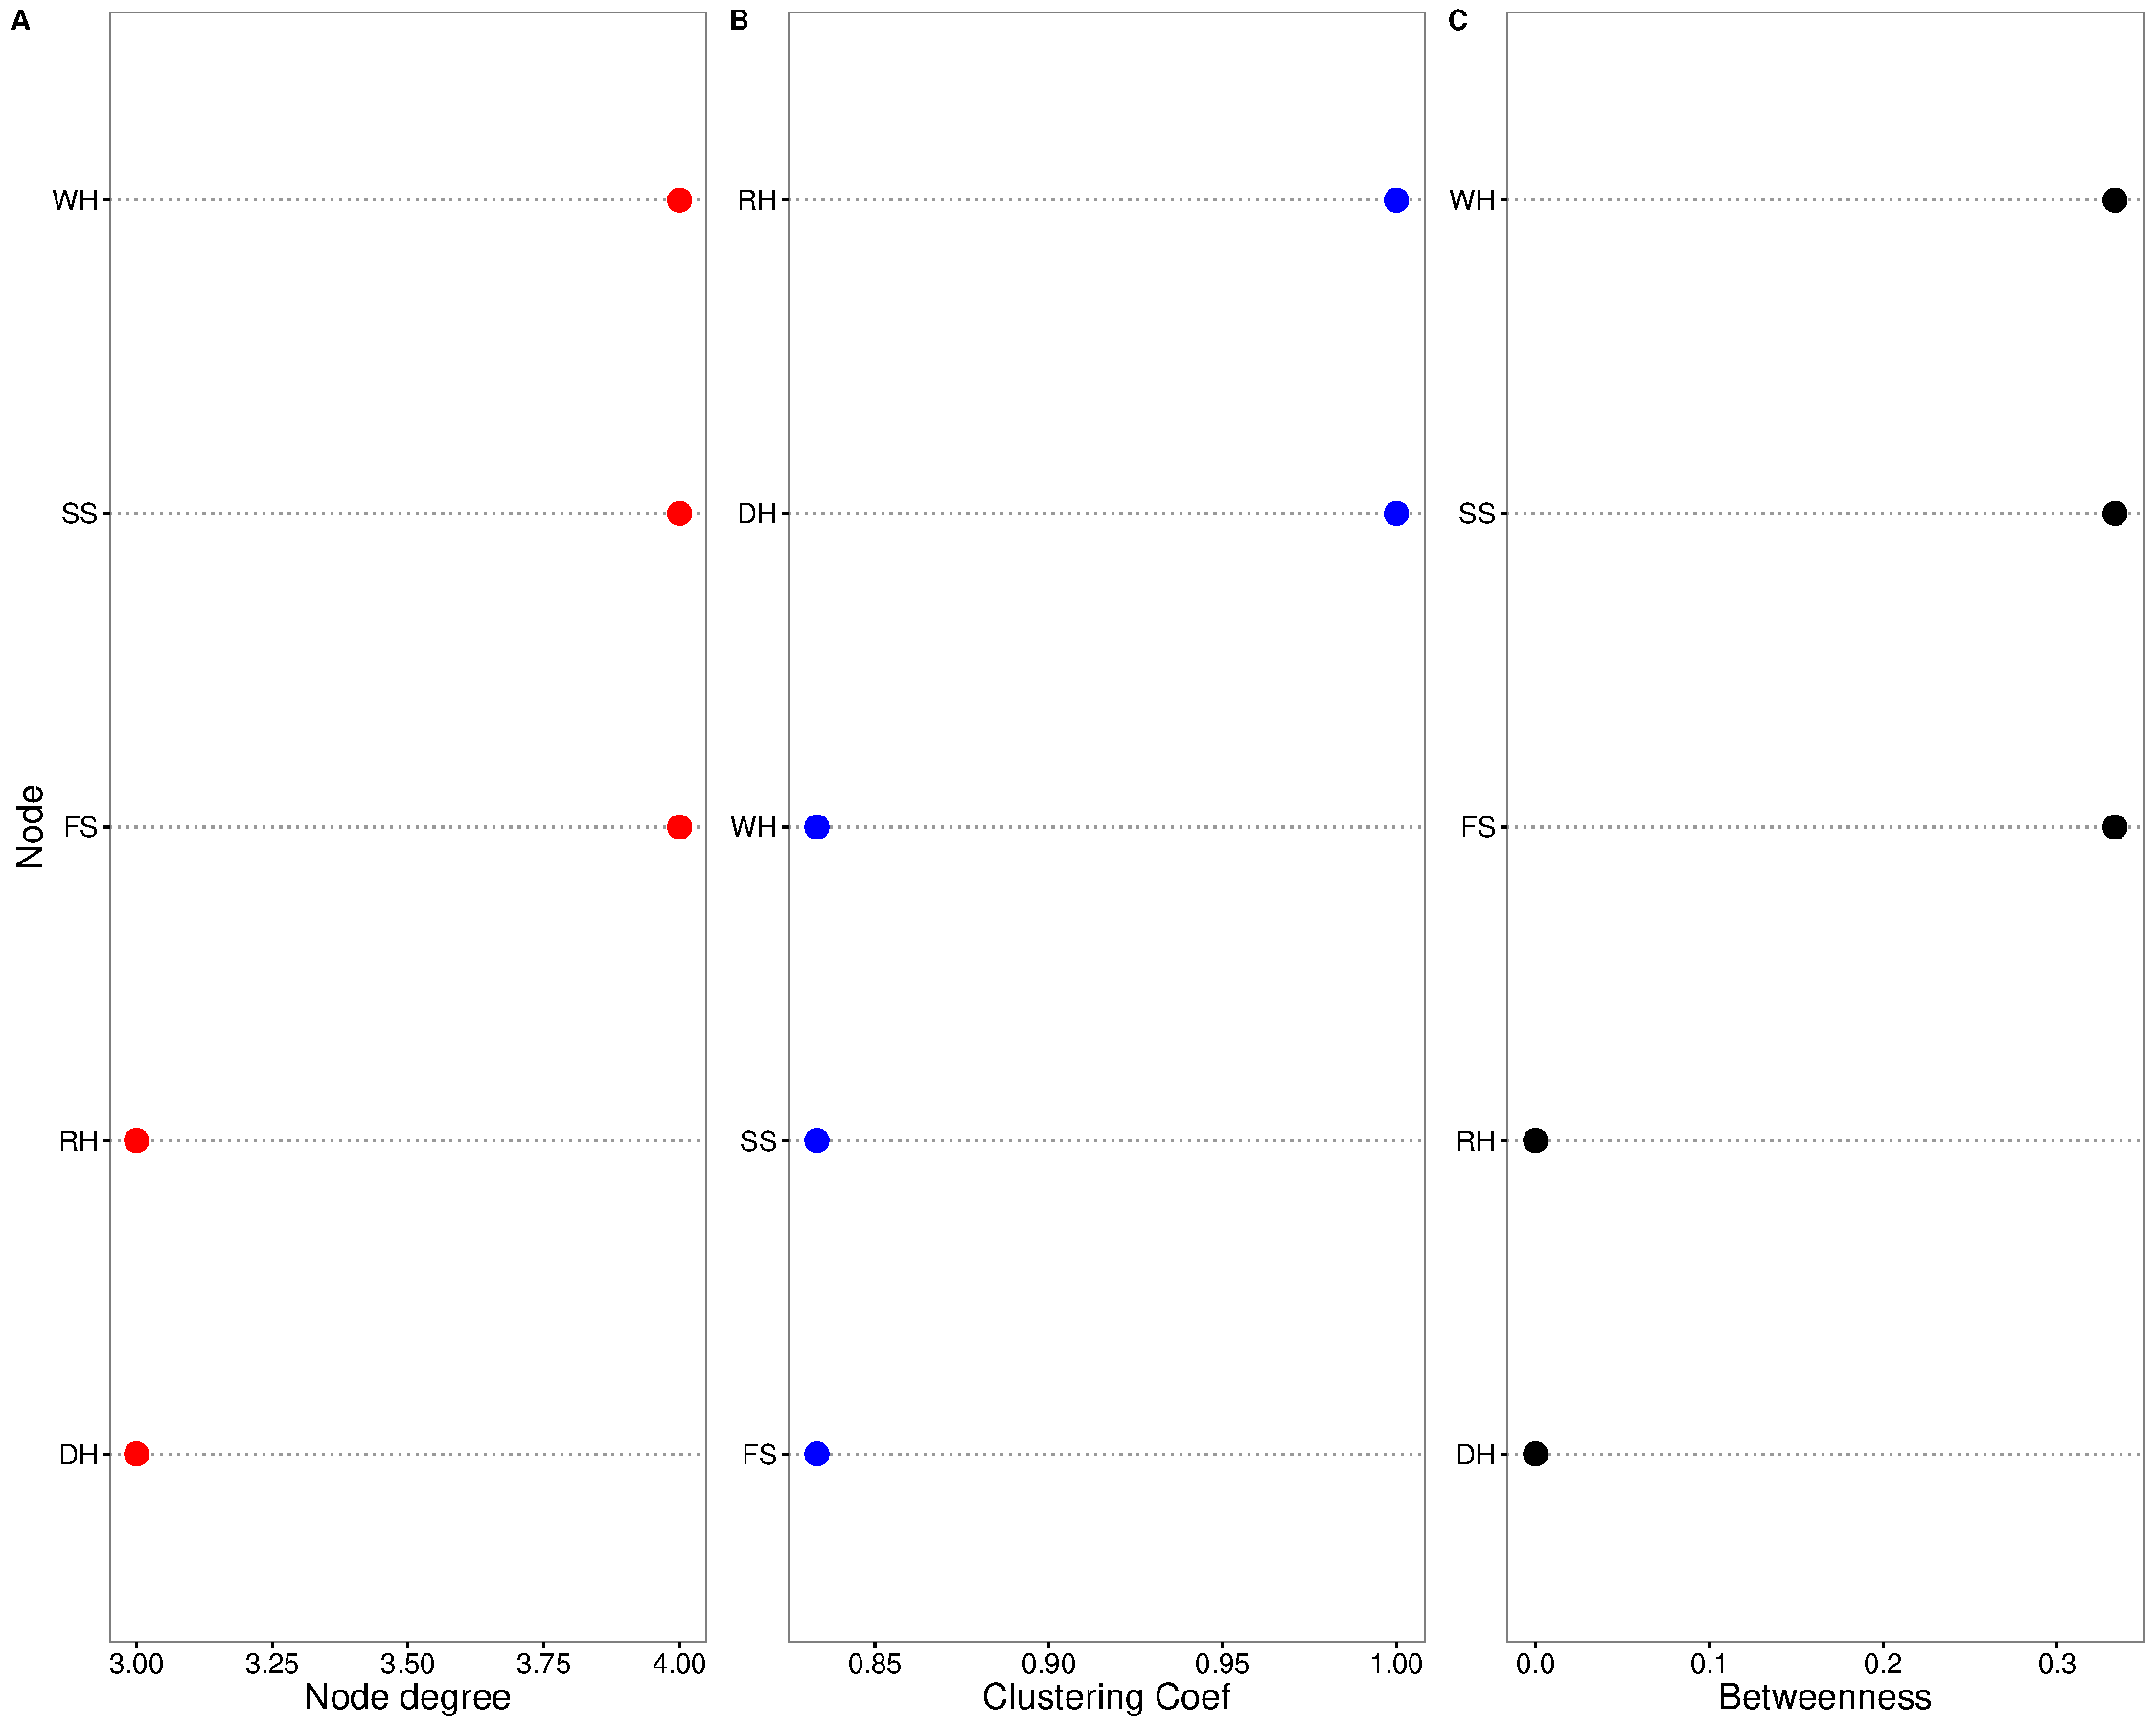
\includegraphics[width = 1\textwidth]{figures/yield_dif_nodepropOdisha.pdf}
        \caption{Three centrality measures of the nodes in co-occurrence network of rice injuries in dry season at Central Plain. A: node degree, B:clustering coefficient, and C:Betweenness.}
        \label{fig:nodepropdifyield_OD}
    \end{subfigure}
    \caption{Rice injuries in dry season in Central Plain, Thailand}
    \label{fig:difyieldOD}
\end{figure}
 
 \begin{figure}
    \centering
    \begin{subfigure}[b]{1\textwidth}
        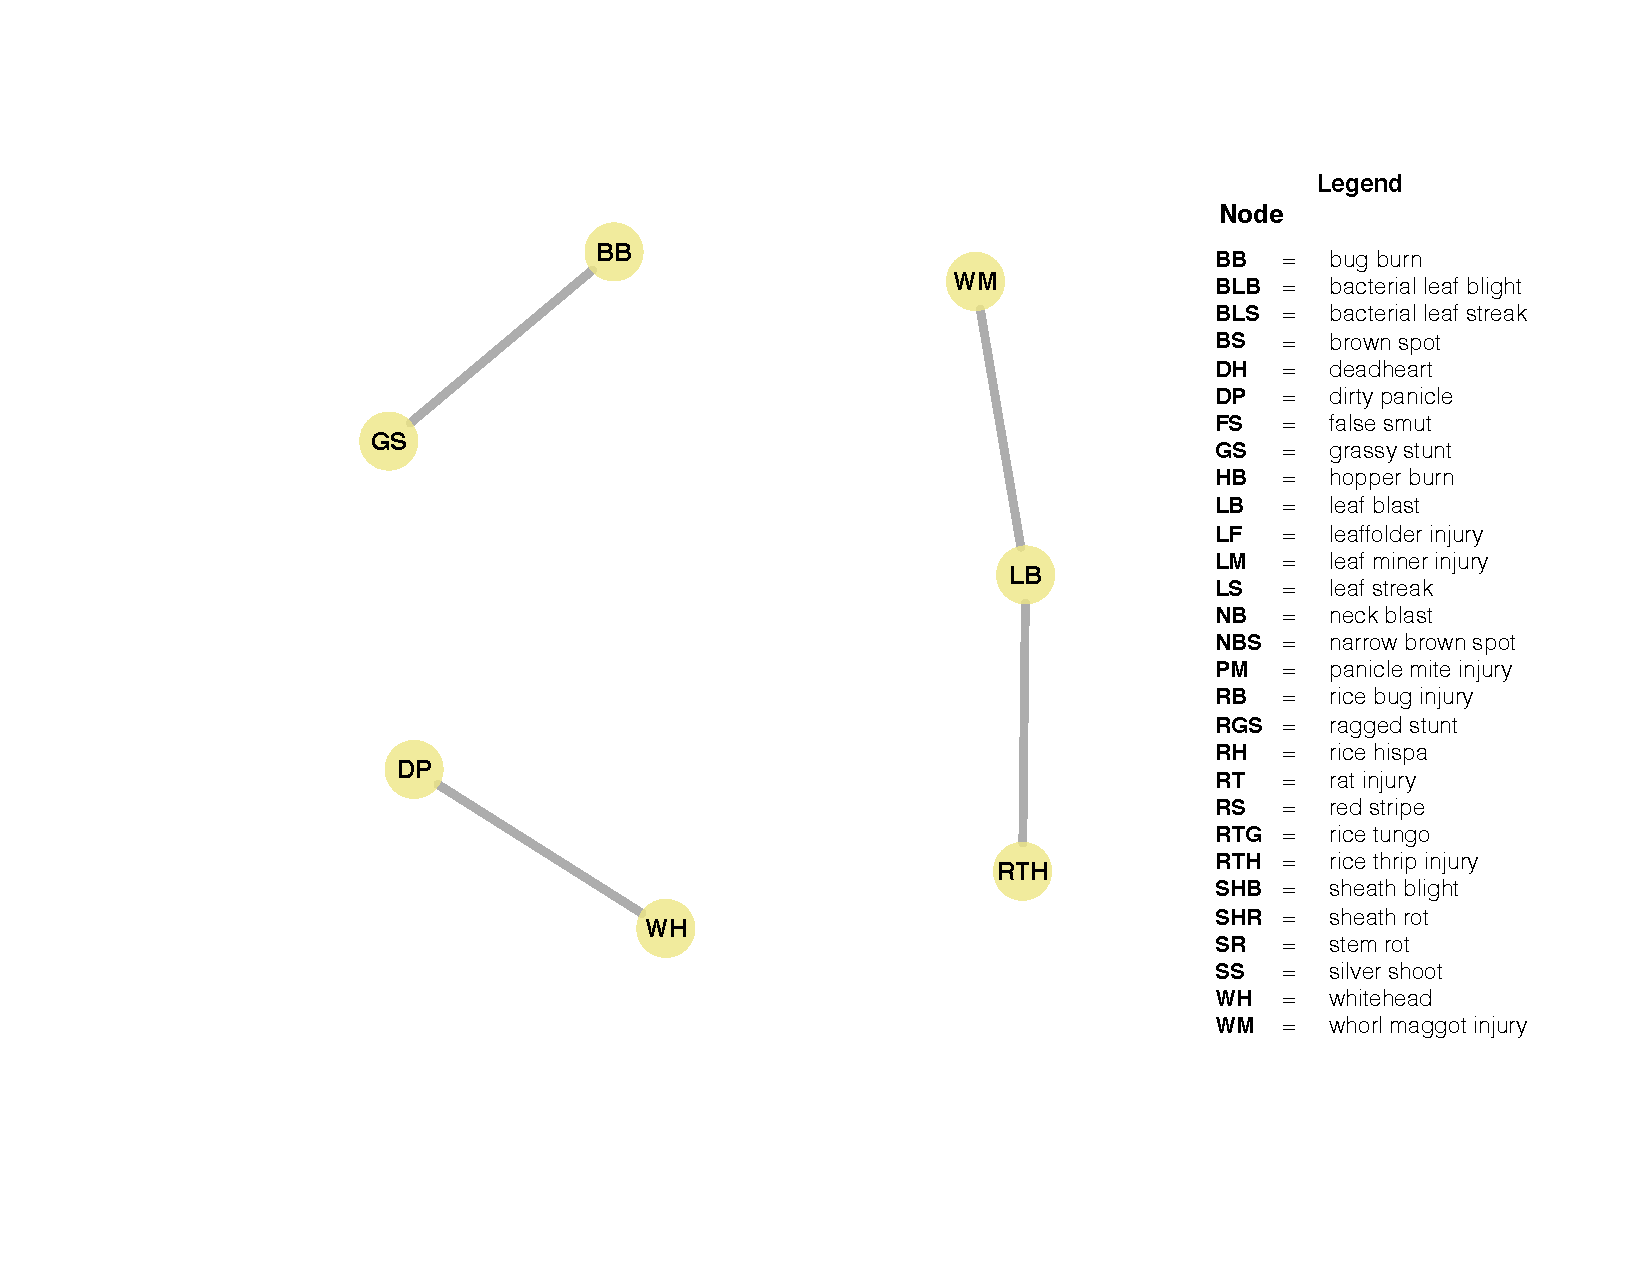
\includegraphics[width = 1\textwidth]{figures/difyieldRR.pdf}
        \caption{Differential co-occurrence network of rice injuries in different yield levels at Central Plain, Thailand. The layout of the network graph is based on the Fruchterman-Reingold algorithm, which places nodes with stronger or more connections closer to each other.}
        \label{fig:difyieldRR}
    \end{subfigure}
    \begin{subfigure}[b]{1\textwidth}
        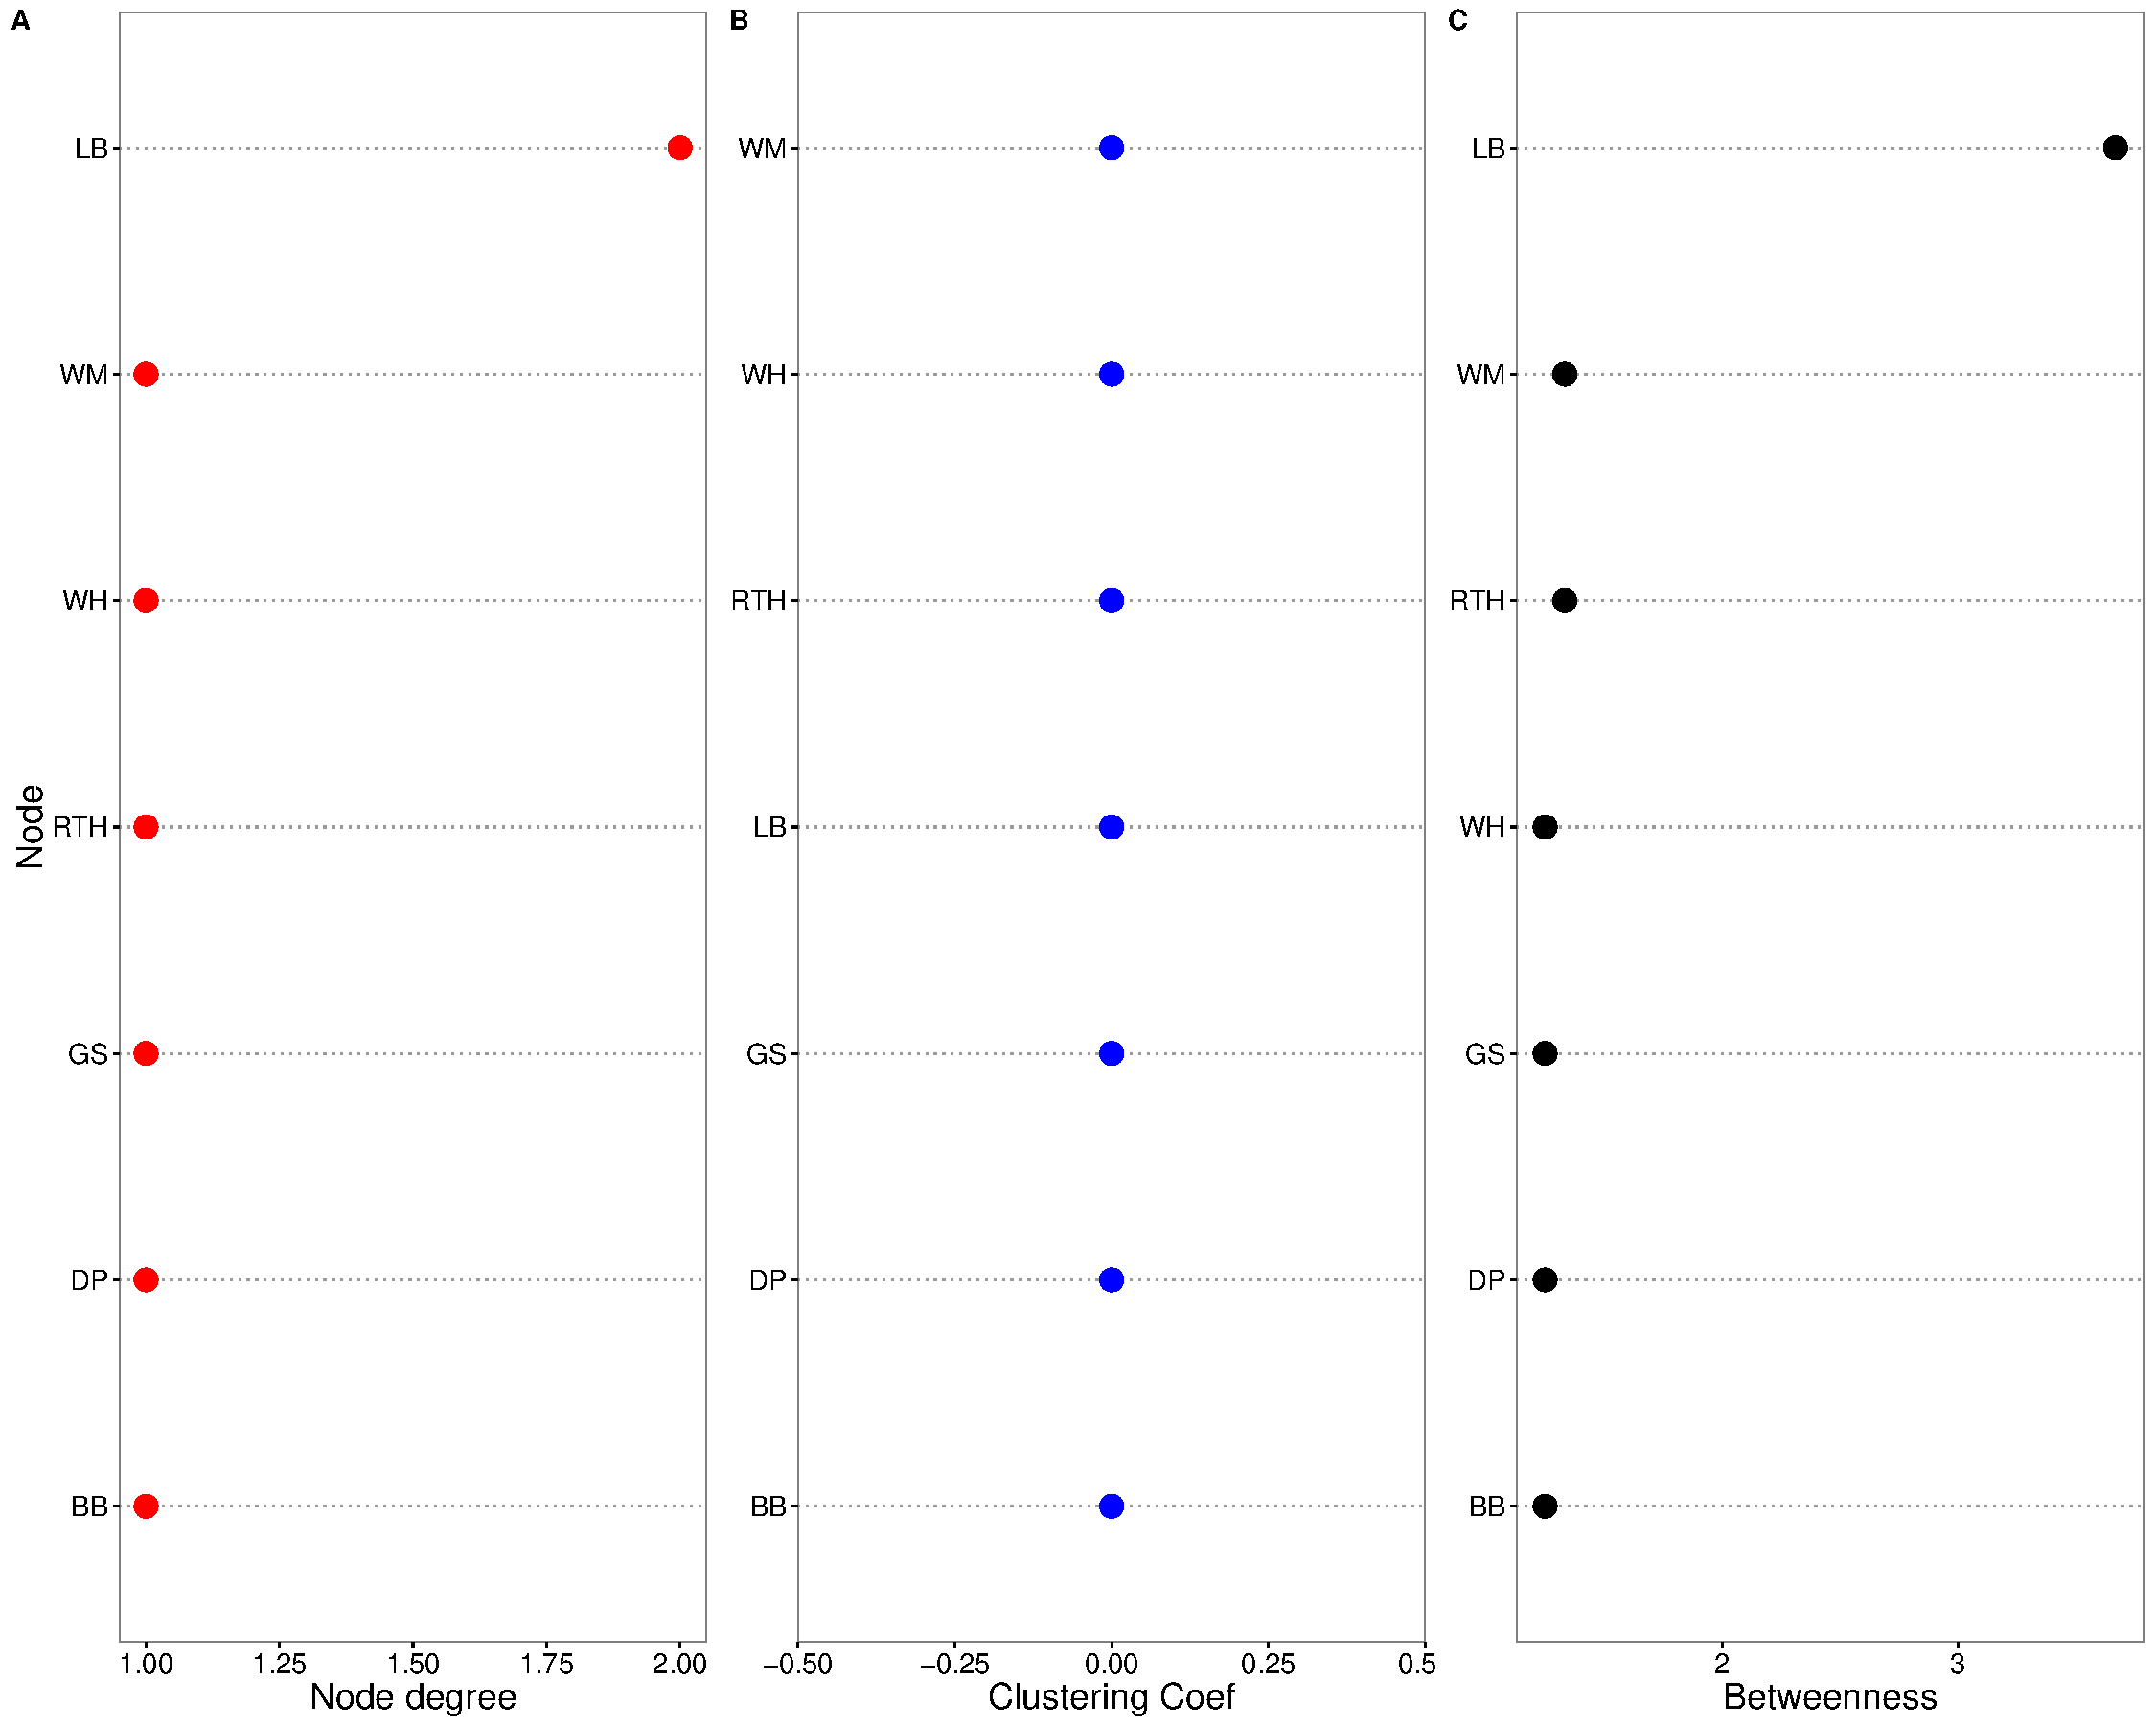
\includegraphics[width = 1\textwidth]{figures/yield_dif_nodepropRed_River_Delta.pdf}
        \caption{Three centrality measures of the nodes in co-occurrence network of rice injuries in dry season at Central Plain. A: node degree, B:clustering coefficient, and C:Betweenness.}
        \label{fig:nodepropdifyield_RR}
    \end{subfigure}
    \caption{Rice injuries in dry season in Central Plain, Thailand}
    \label{fig:CP_ds}
\end{figure}
 
 \begin{figure}
    \centering
    \begin{subfigure}[b]{1\textwidth}
        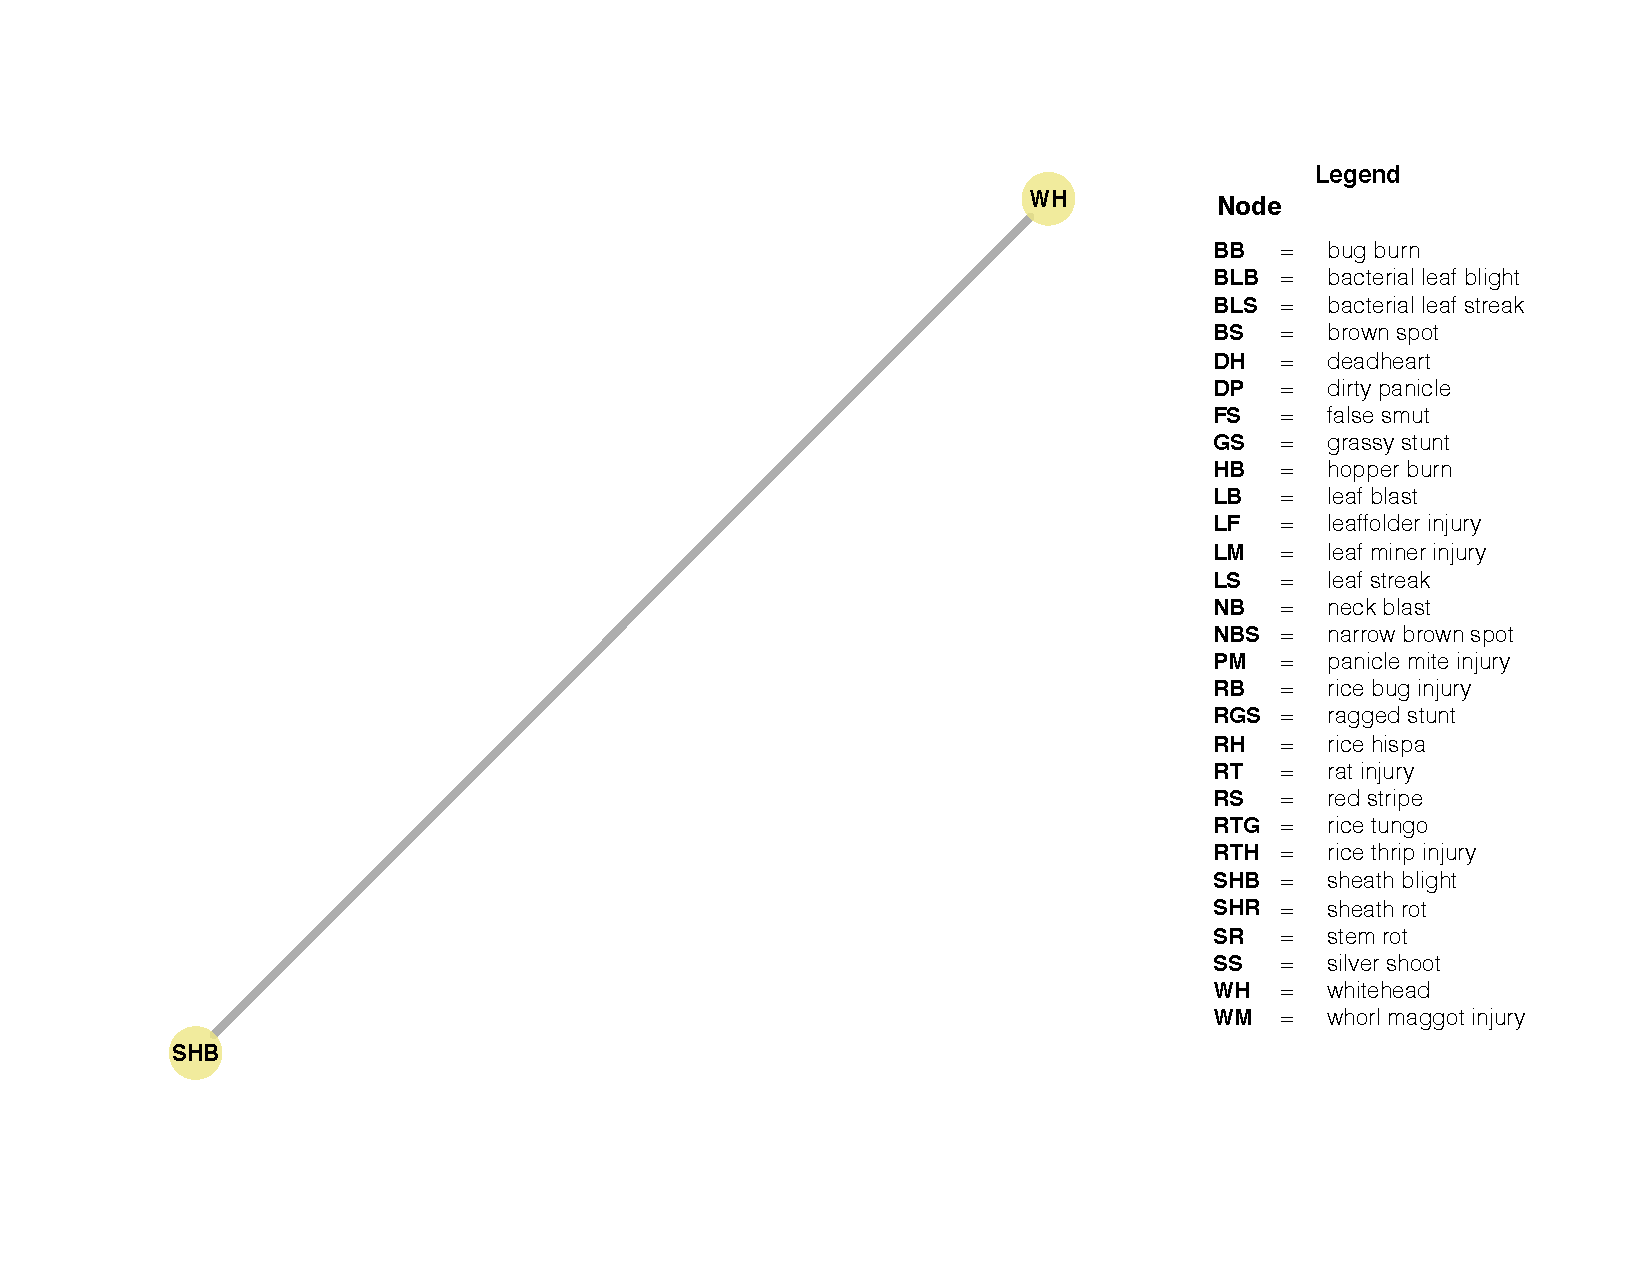
\includegraphics[width = 1\textwidth]{figures/difyieldTM.pdf}
        \caption{Differential co-occurrence network of rice injuries in different yield levels at Central Plain, Thailand. The layout of the network graph is based on the Fruchterman-Reingold algorithm, which places nodes with stronger or more connections closer to each other.}
        \label{fig:difyield_WJ}
    \end{subfigure}
    \begin{subfigure}[b]{1\textwidth}
        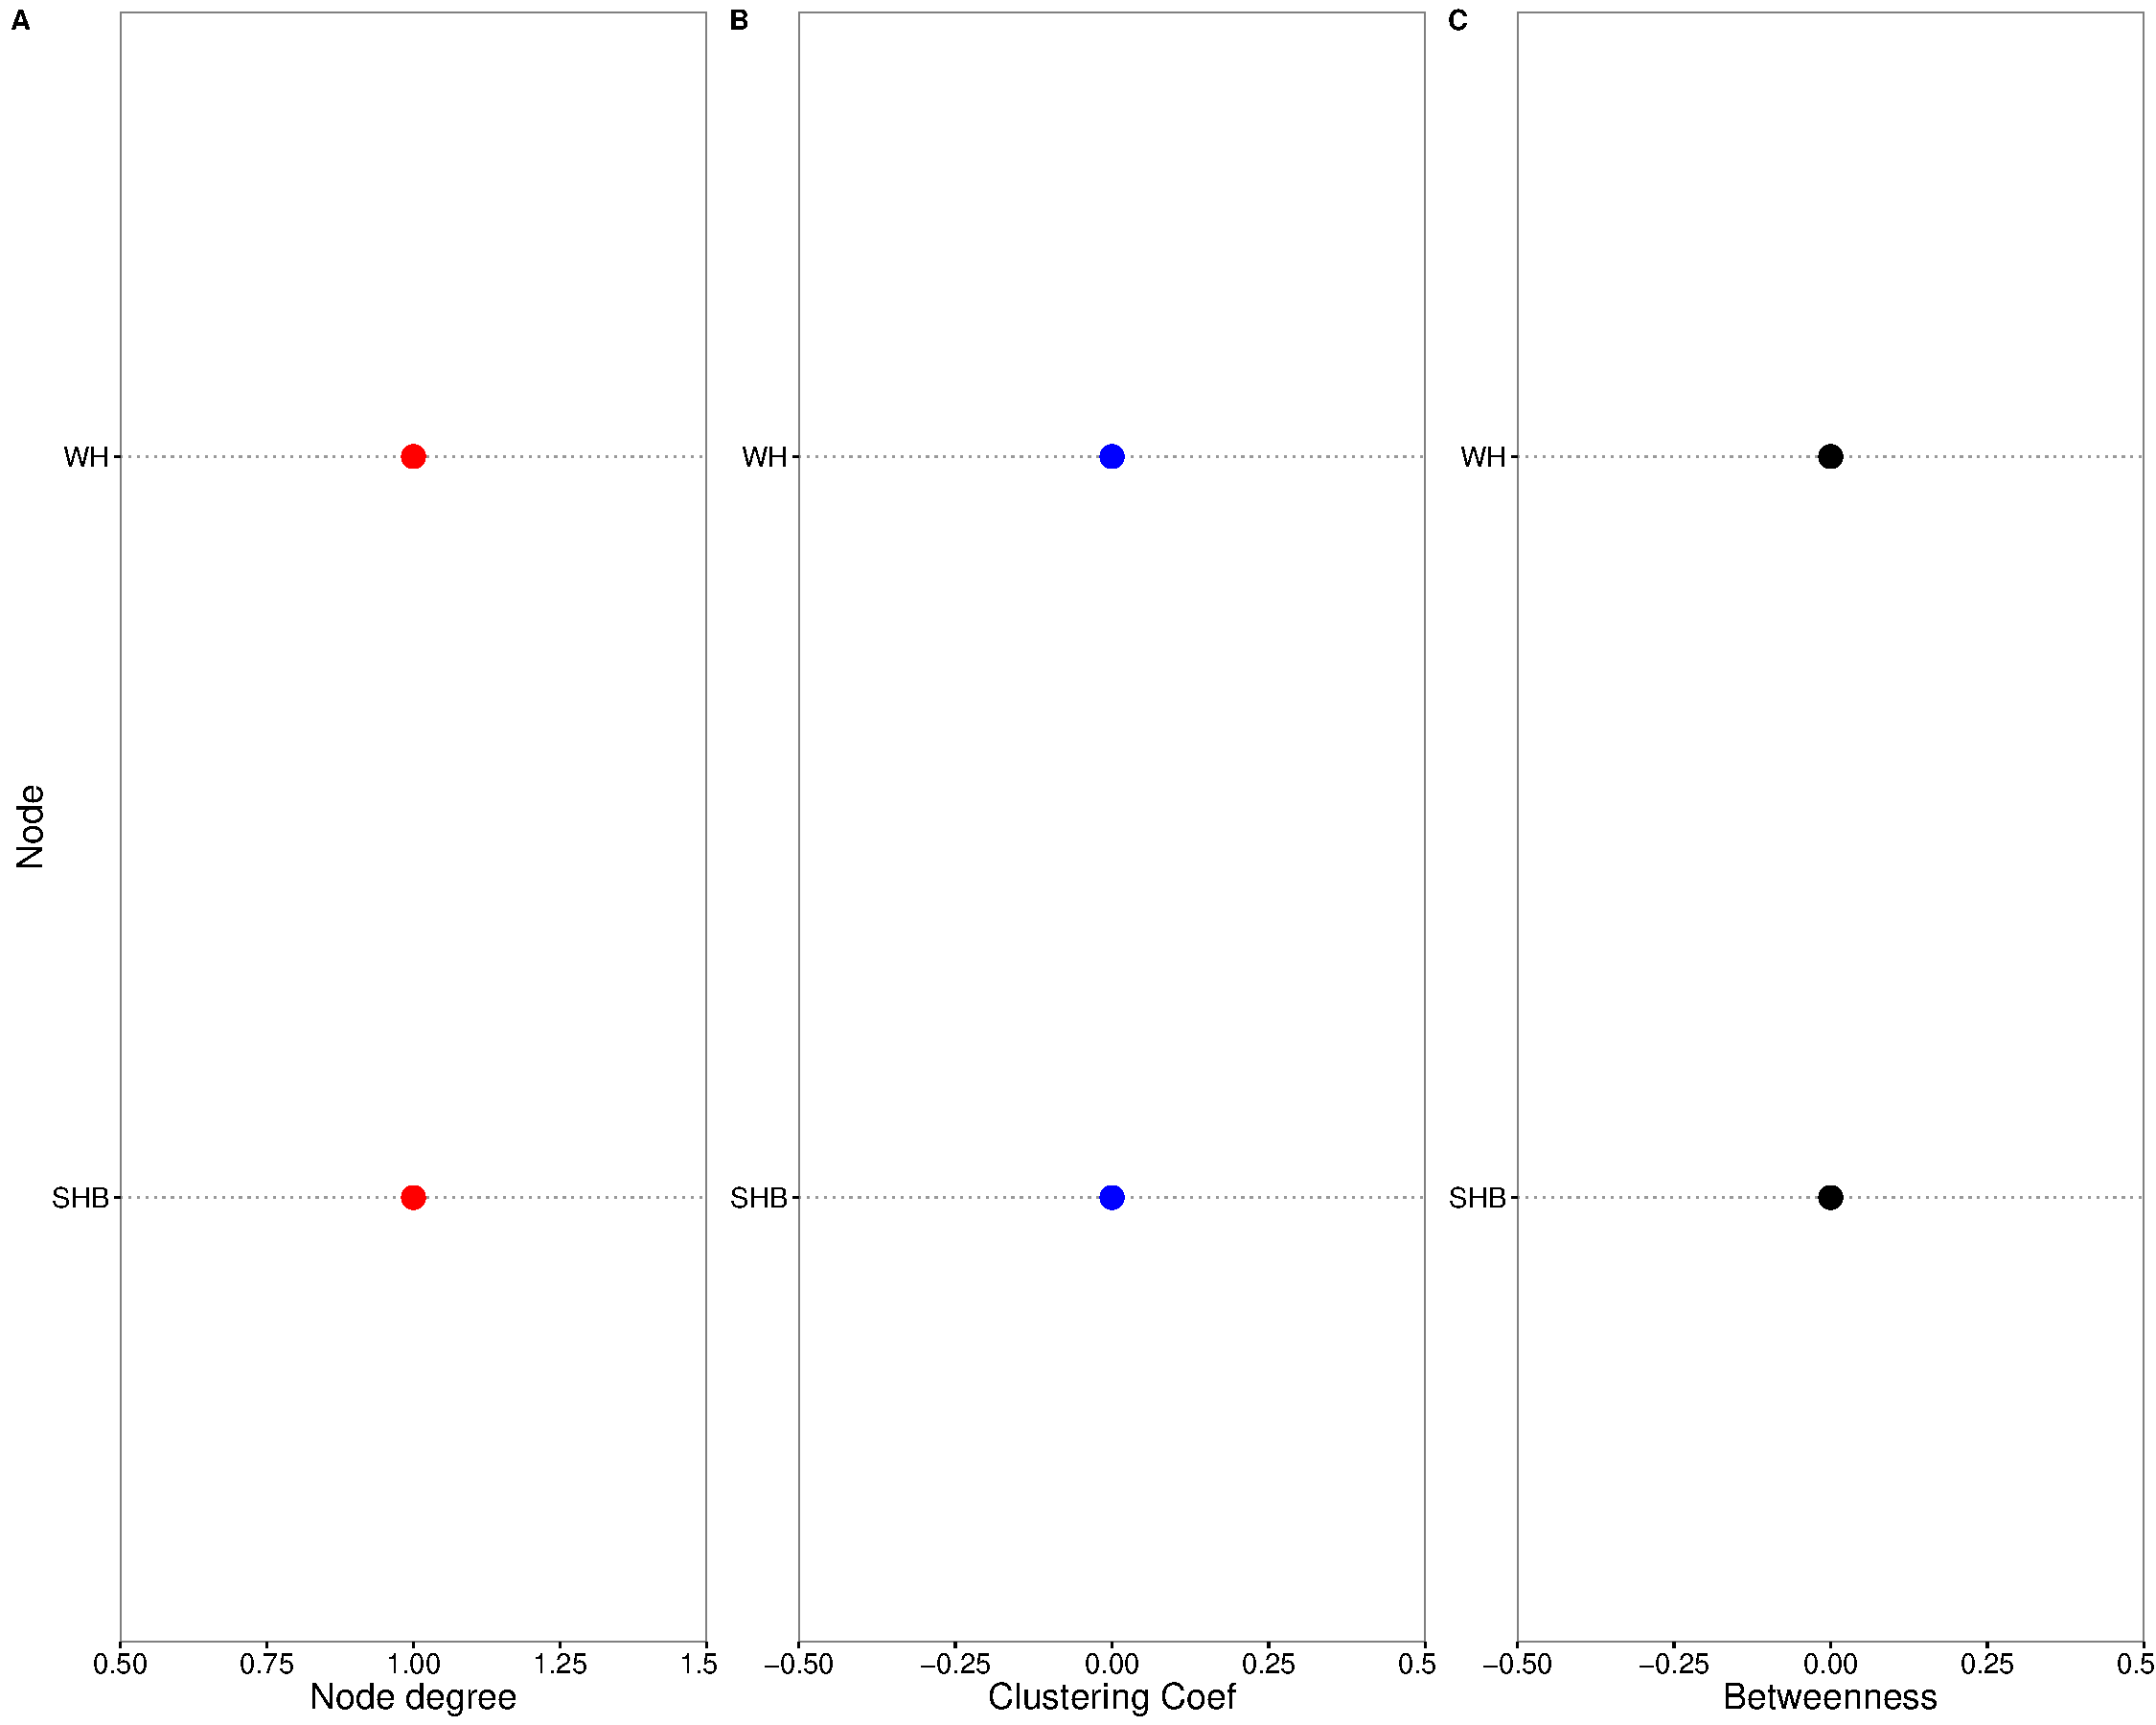
\includegraphics[width = 1\textwidth]{figures/yield_dif_nodepropTamil_Nadu.pdf}
        \caption{Three centrality measures of the nodes in co-occurrence network of rice injuries in dry season at Central Plain. A: node degree, B:clustering coefficient, and C:Betweenness.}
        \label{fig:nodepropdifyield_WJ}
    \end{subfigure}
    \caption{.}
    \label{fig:nodeprop_yielddif_WJ}
\end{figure}

% ===
\begin{figure}
    \centering
        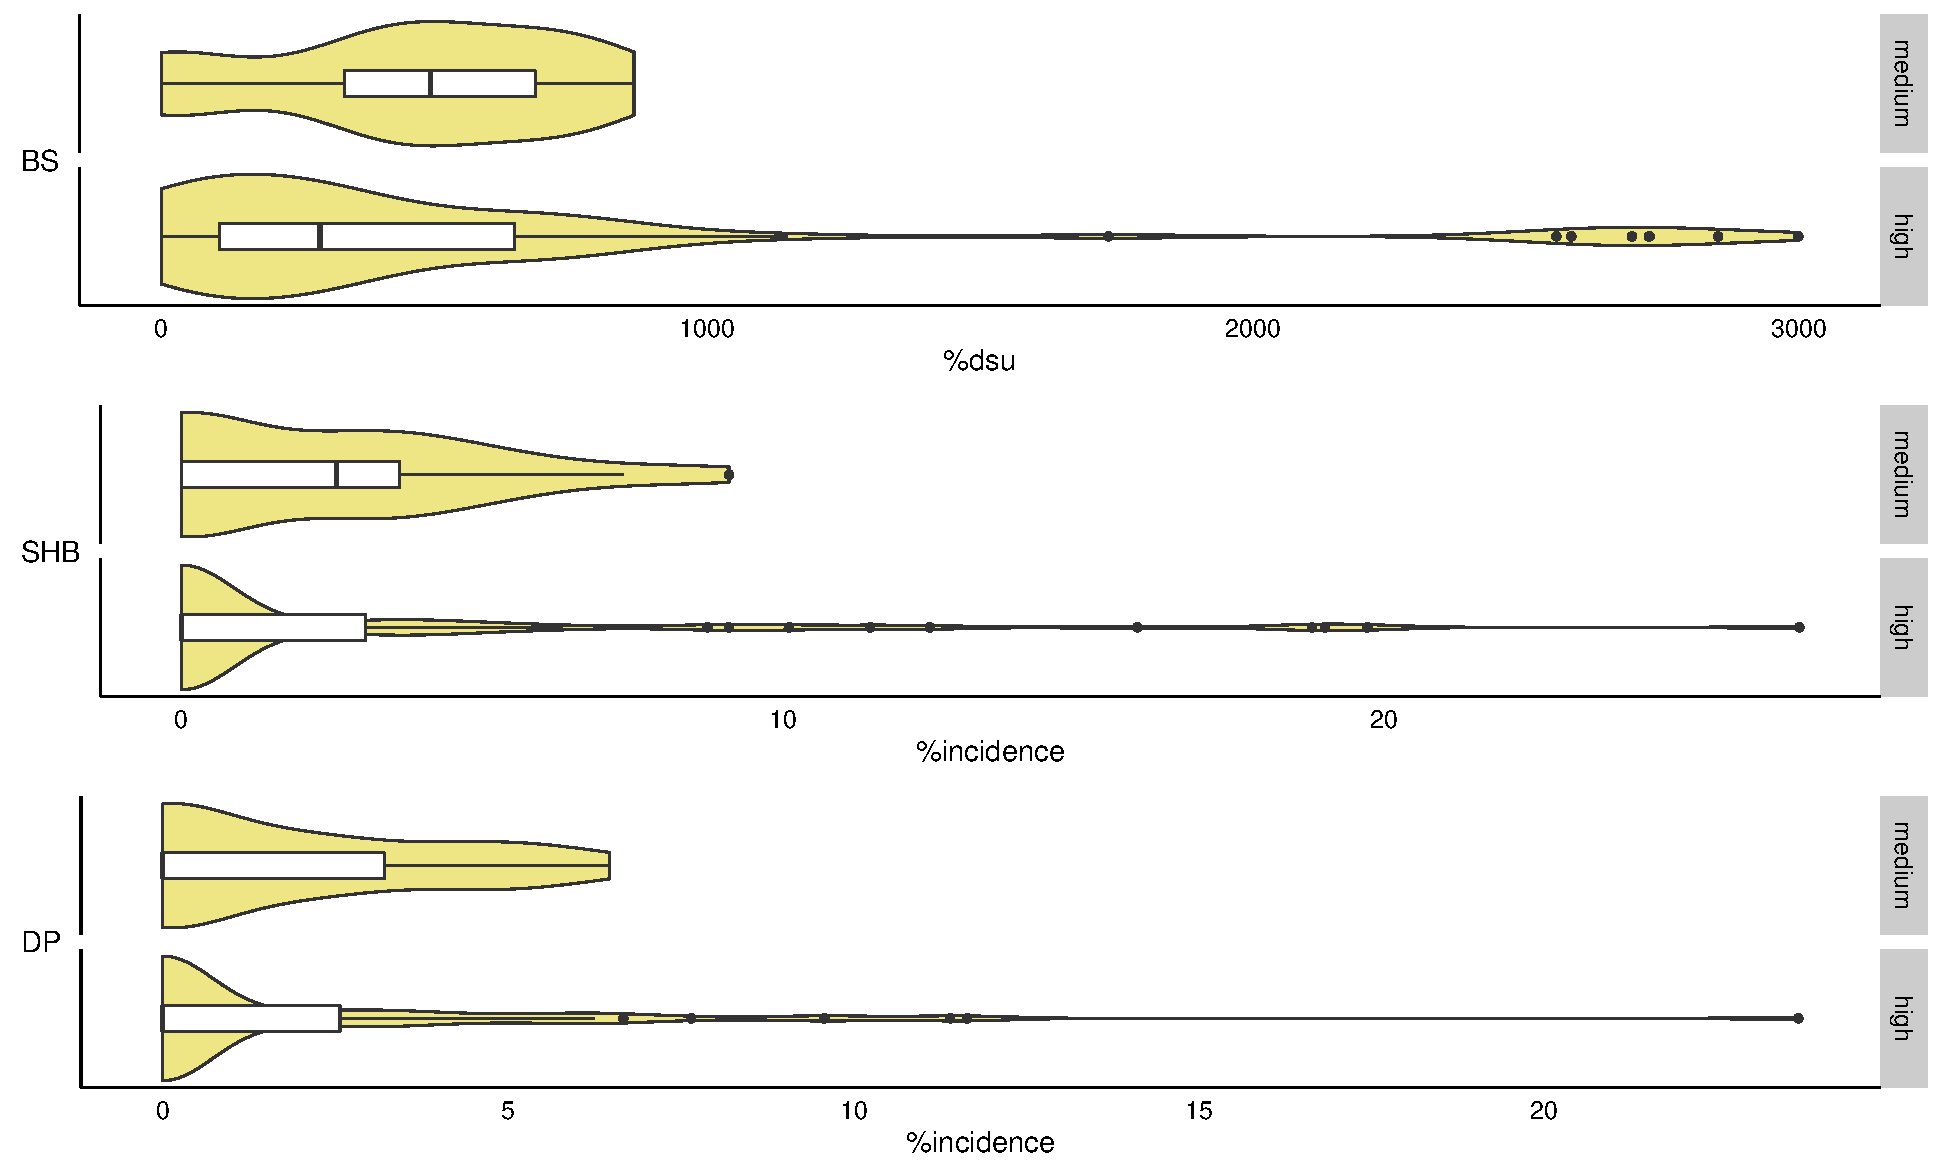
\includegraphics[width = 1\textwidth]{figures/CP_yield_box.pdf}
        \caption{.}
        \label{fig:CP.yield.box}
\end{figure}


\begin{figure}
        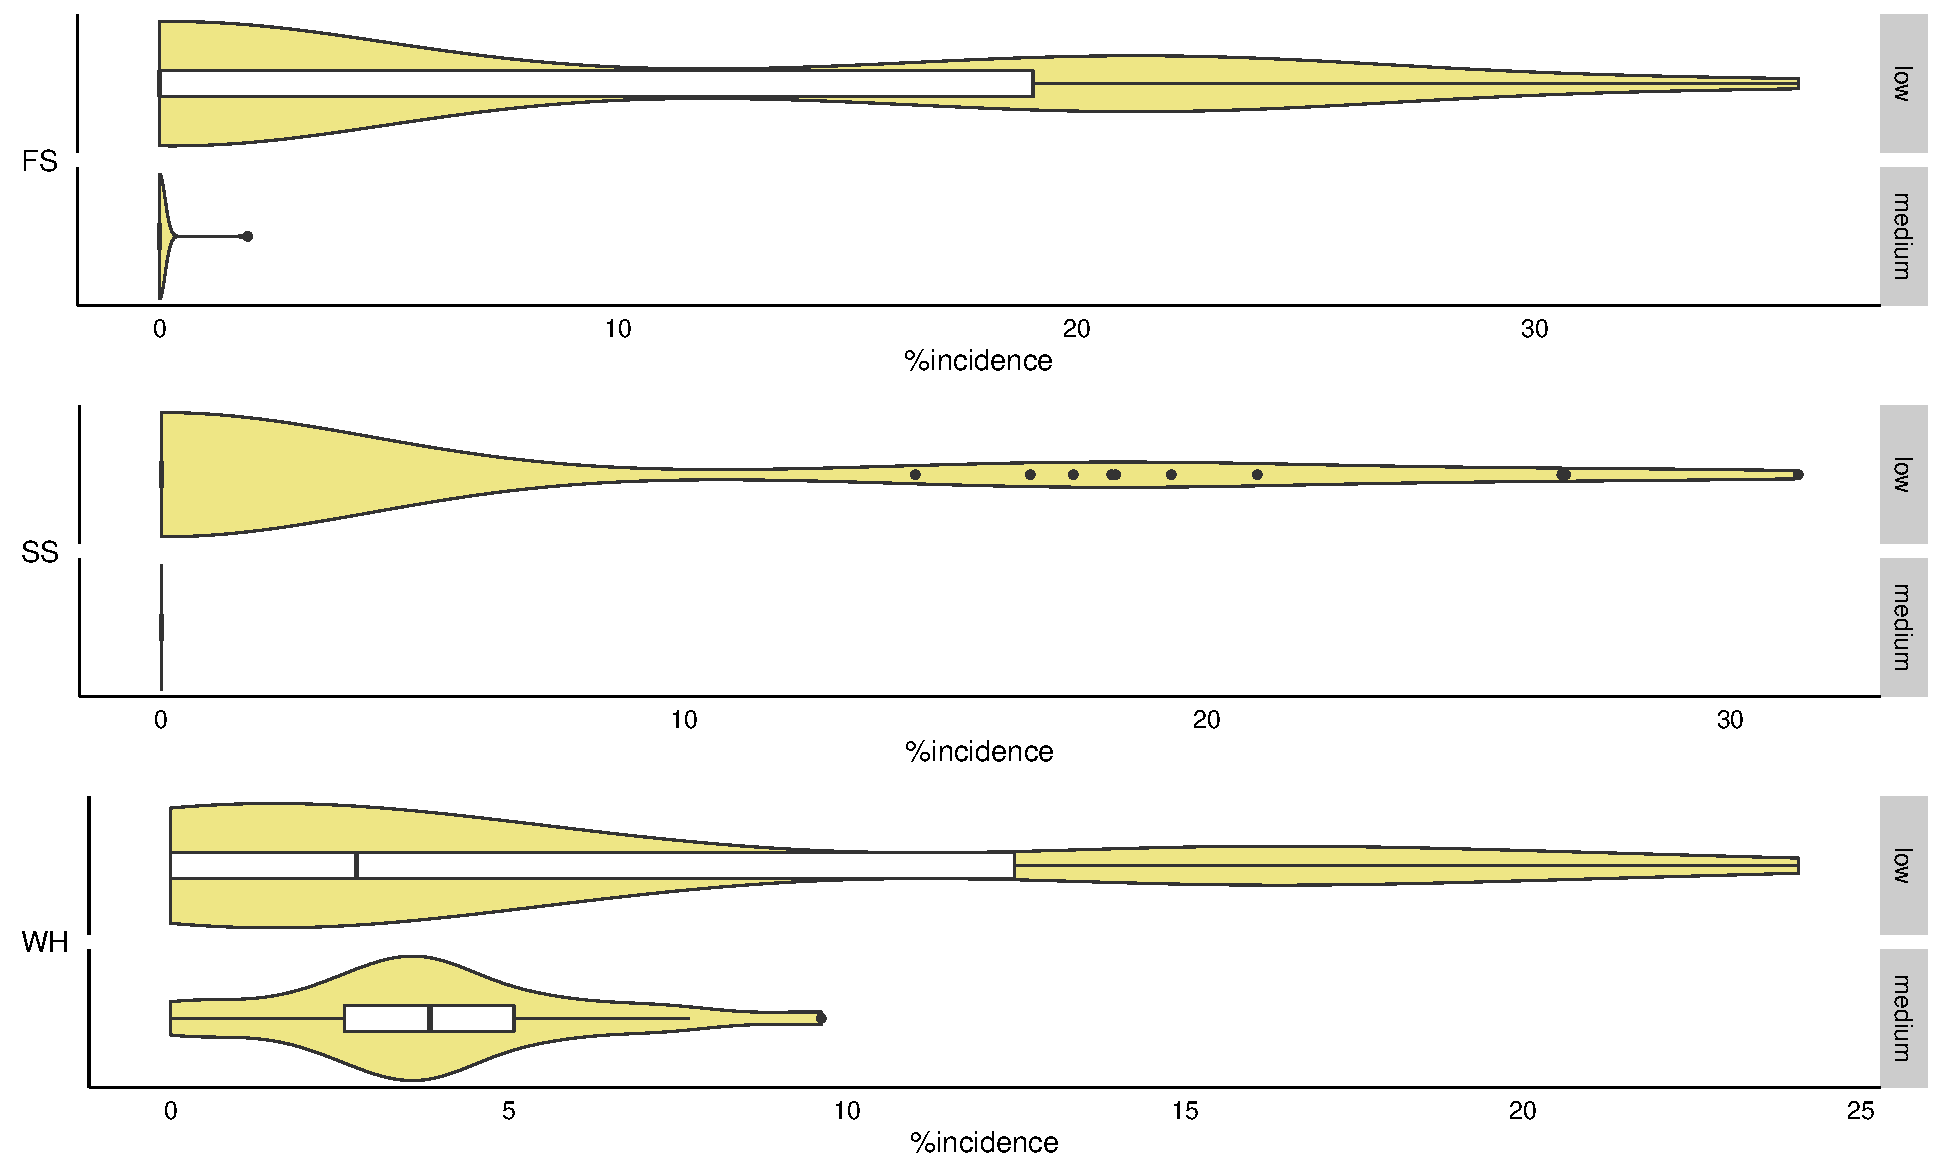
\includegraphics[width = 1\textwidth]{figures/OD_yield_box.pdf}
        \caption{.}
\label{fig:OR.yield.box}
\end{figure}

\begin{figure}
    \centering
        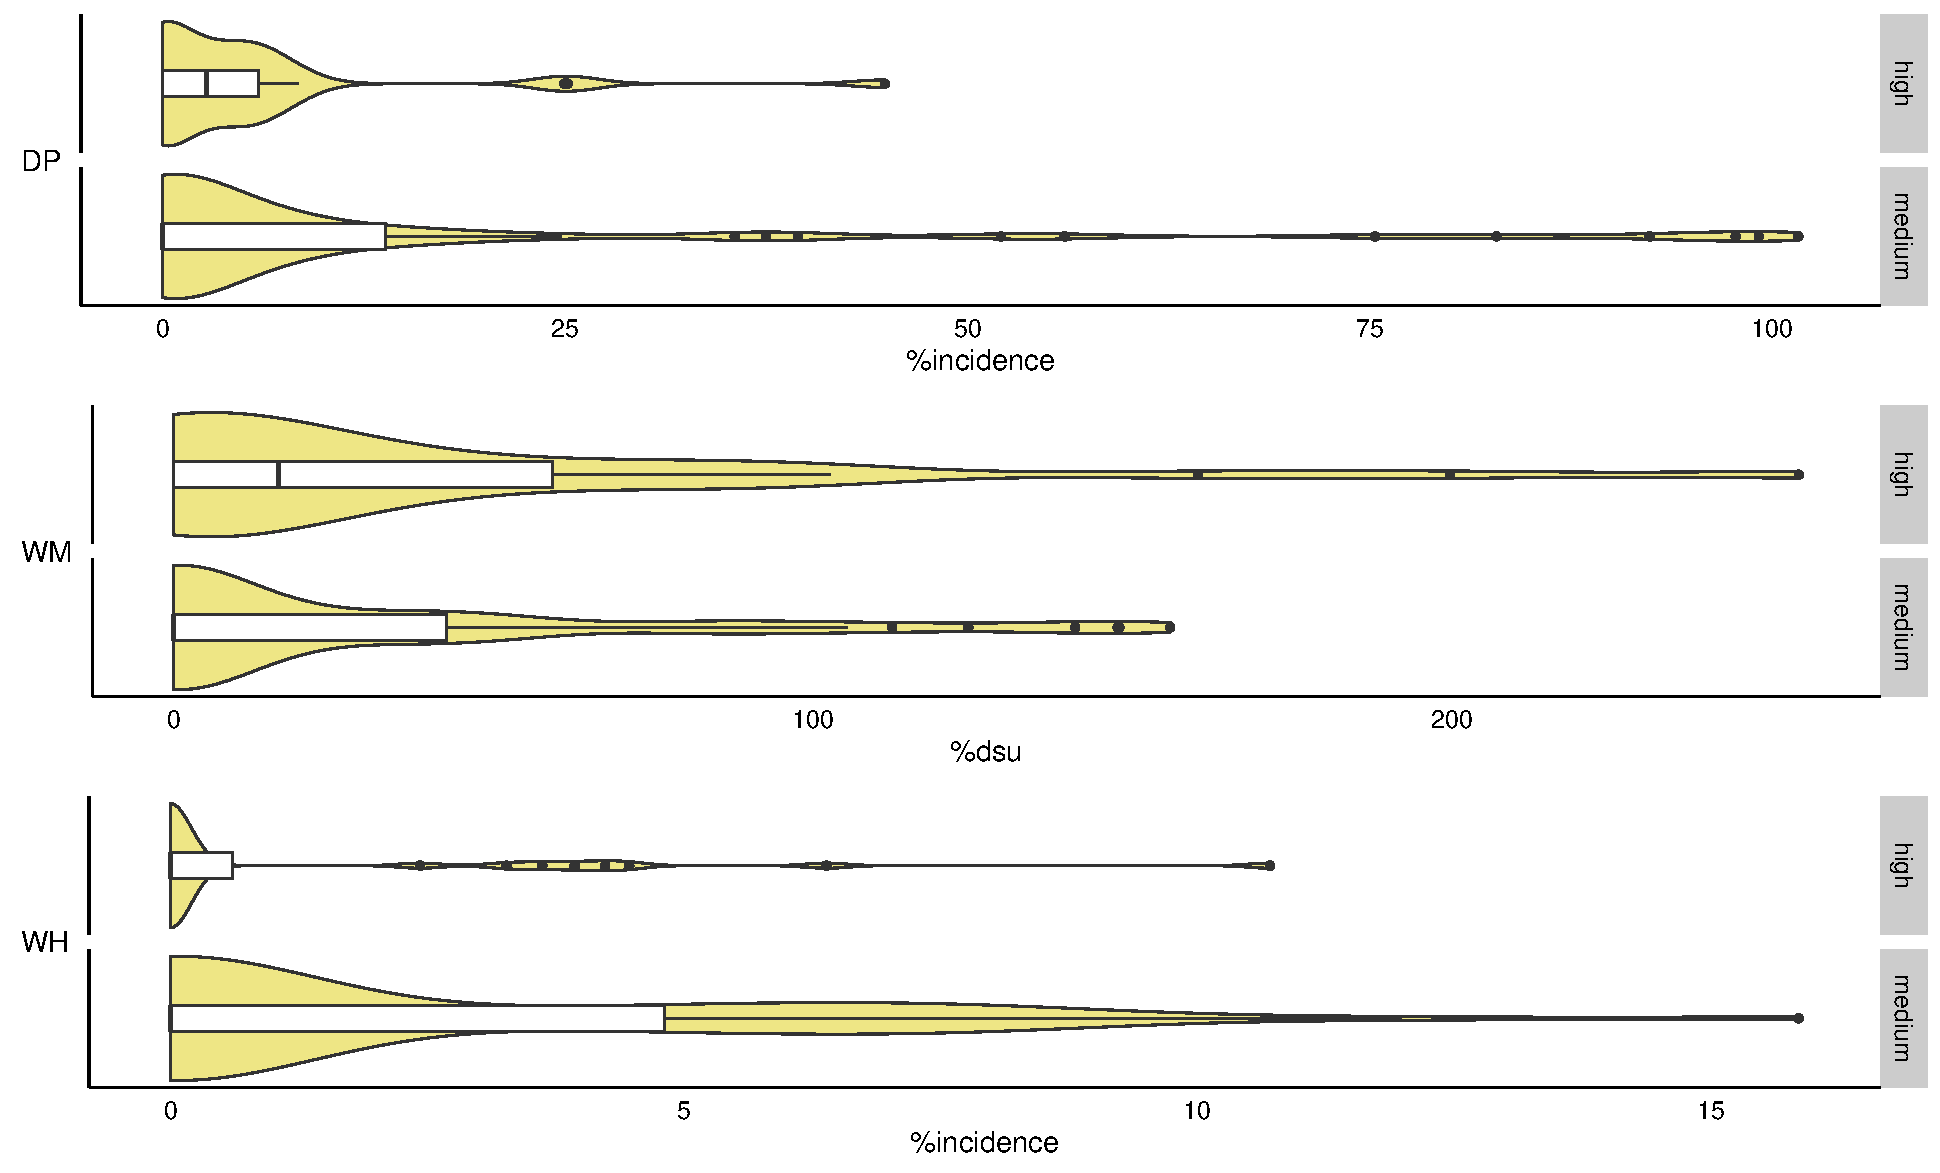
\includegraphics[width = 1\textwidth]{figures/RR_yield_box.pdf}
        \caption{.}
        \label{fig:CP.yield.box}
\end{figure}


\begin{figure}
        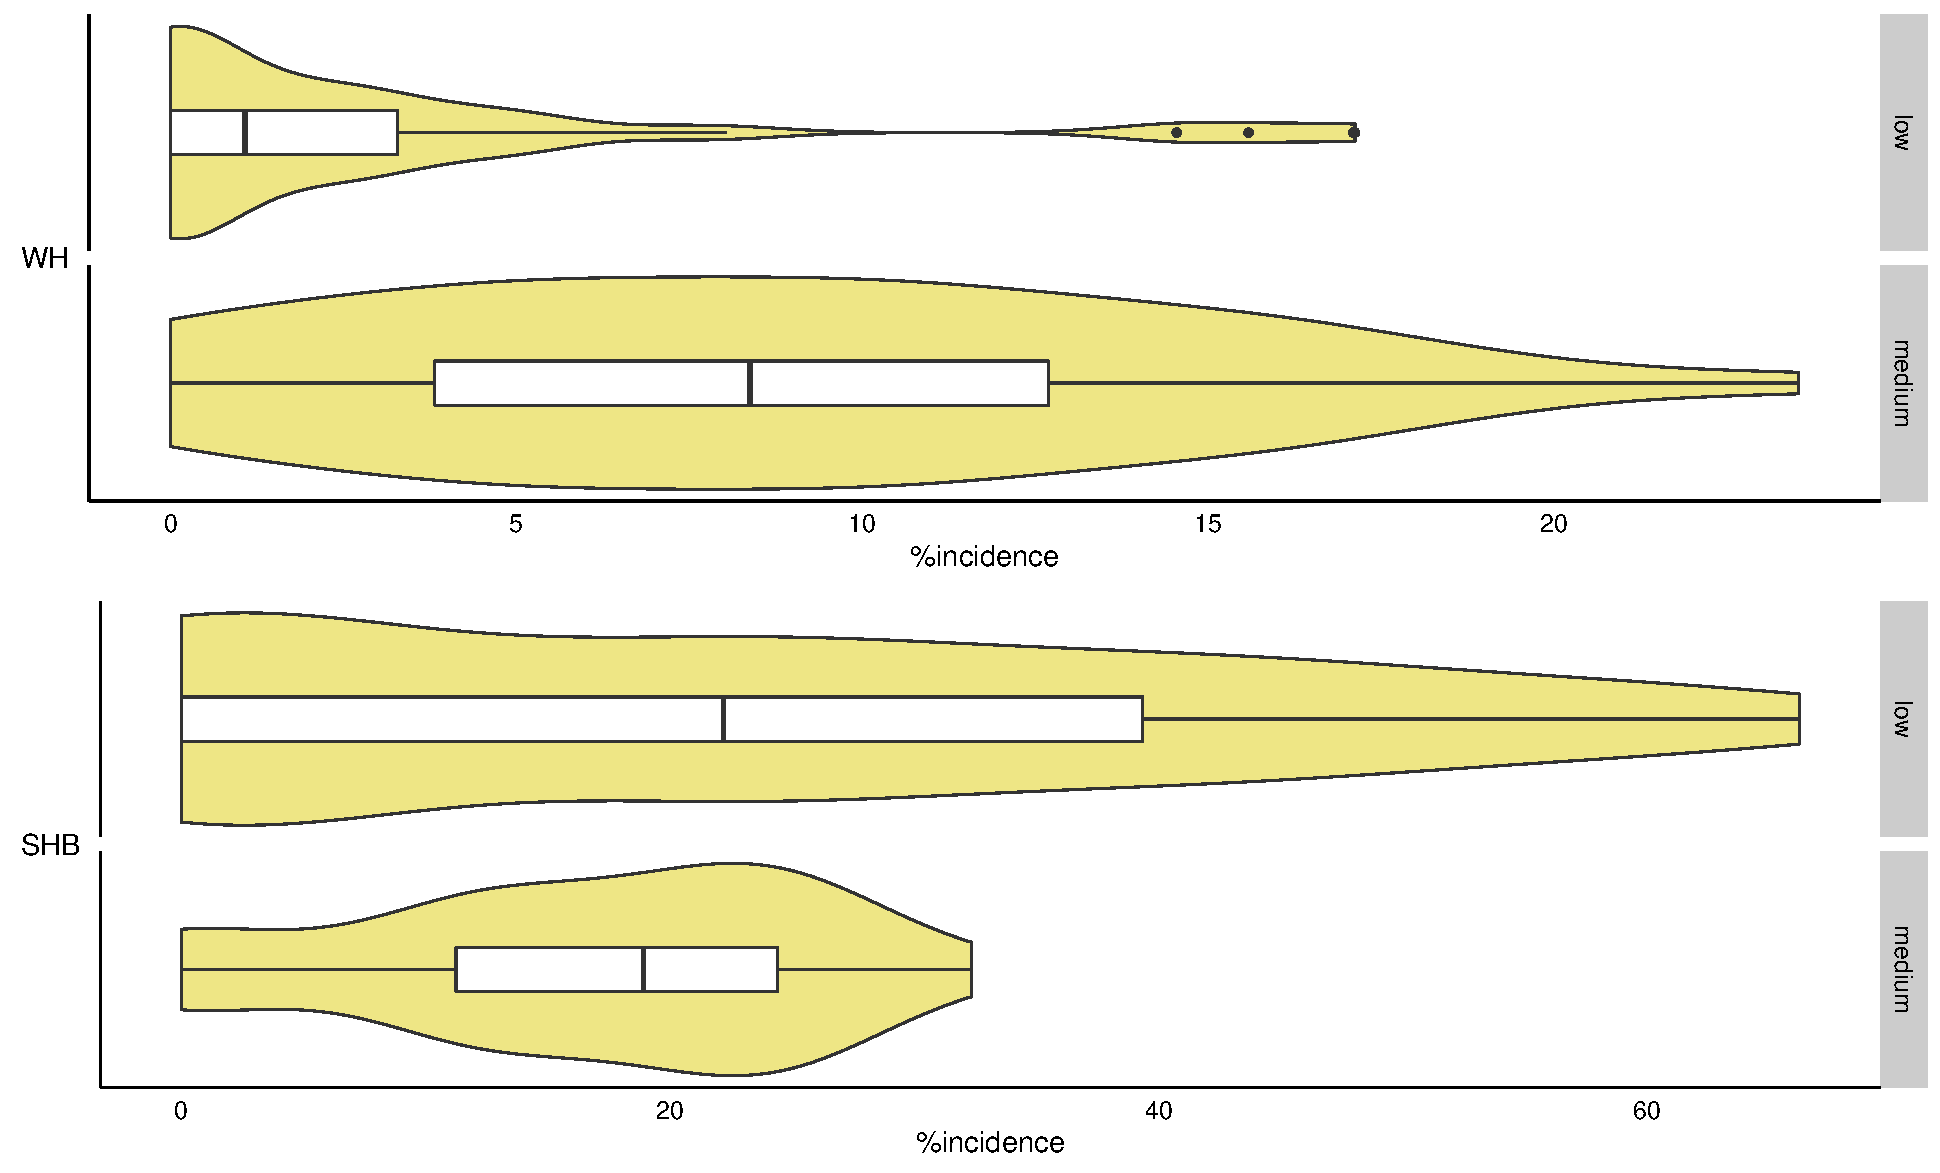
\includegraphics[width = 1\textwidth]{figures/TM_yield_box.pdf}
        \caption{.}
\label{fig:OR.yield.box}
\end{figure}

\begin{figure}
        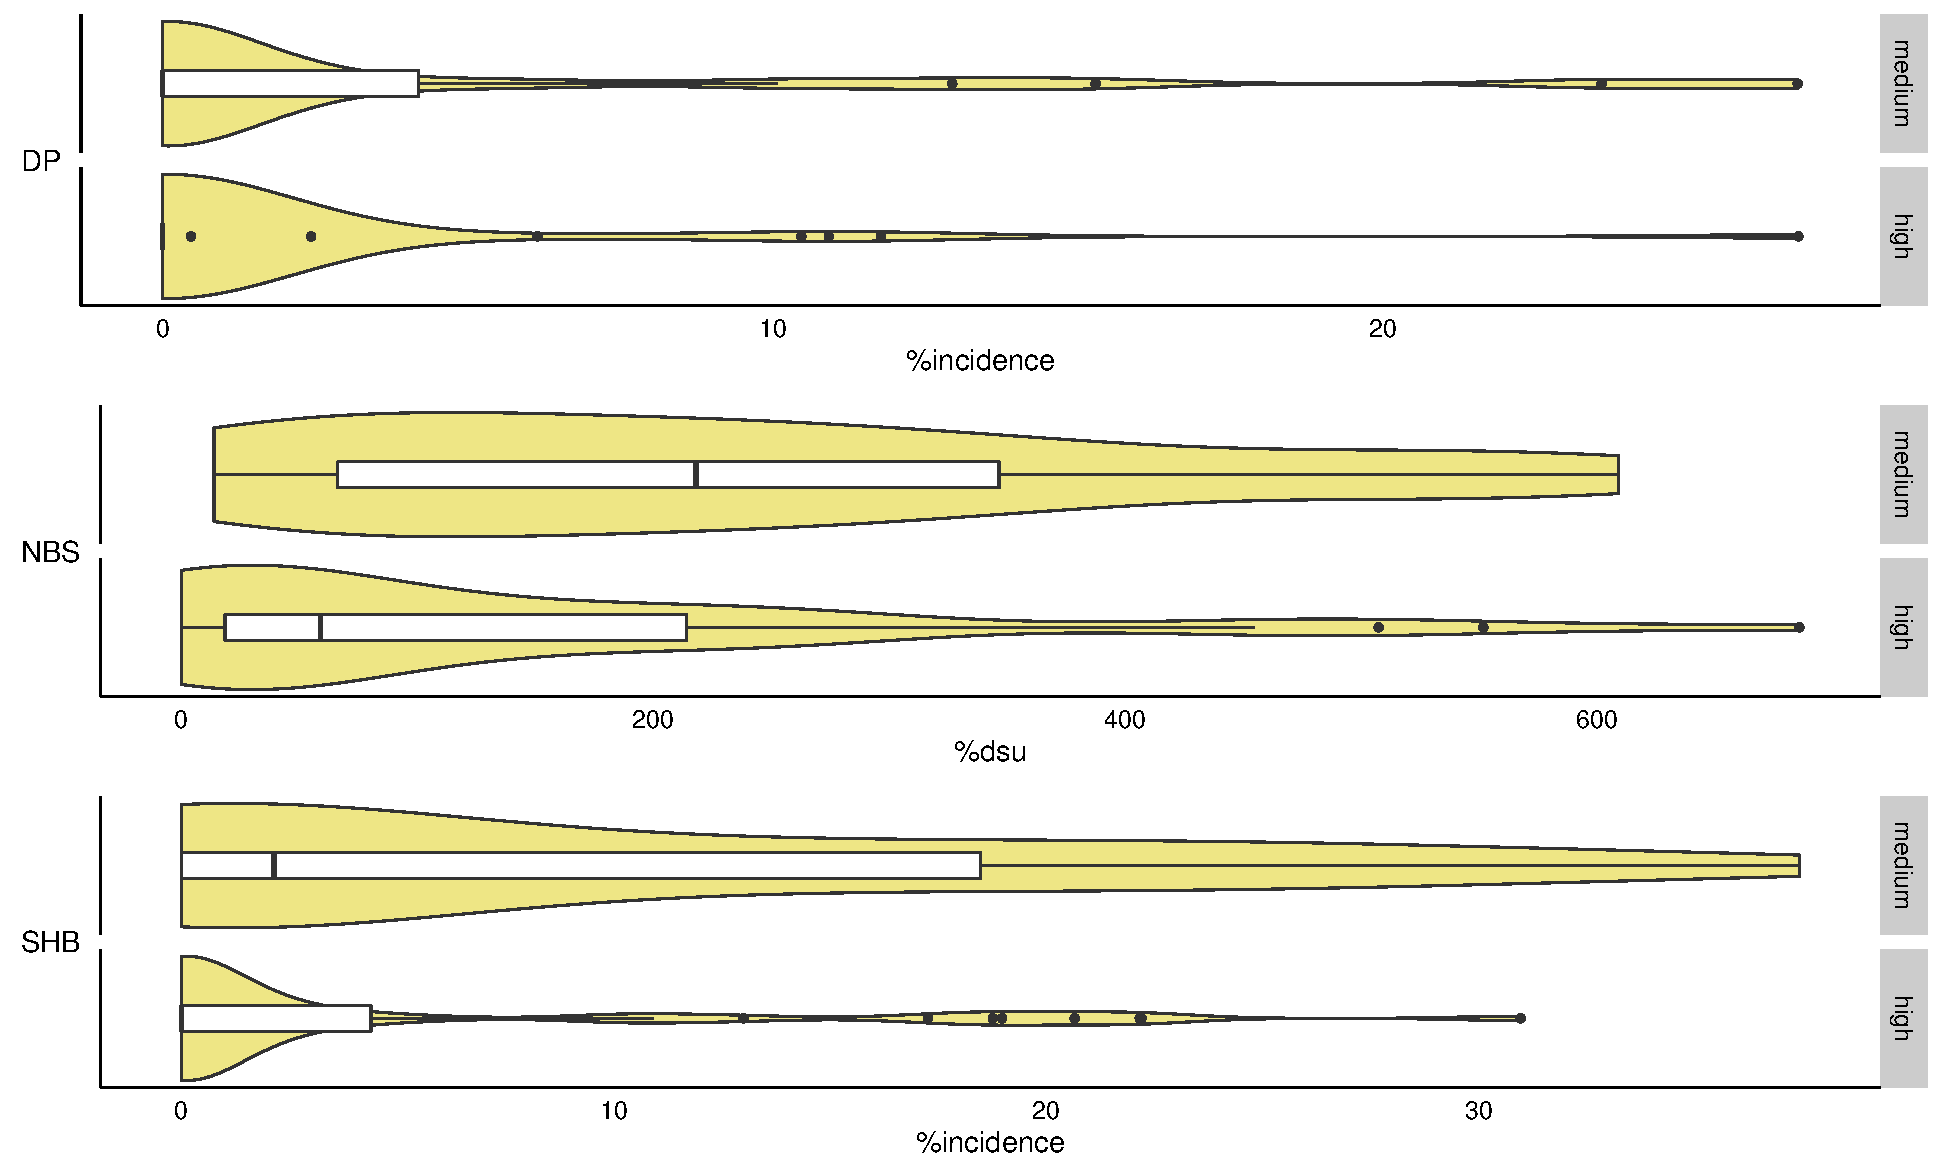
\includegraphics[width = 1\textwidth]{figures/WJ_yield_box.pdf}
        \caption{.}
\label{fig:OR.yield.box}
\end{figure}

\subsection{Discussion}

%Systems biology methods like this are in high demand as the differences between many conditions, be they neurodegenerative diseases, brain diseases, different kinds of cancers, different degrees of disease severity, and so forth, are very subtle and cannot be easily highlighted using the usual off-the-shelf clustering or biological pathways identification algorithms. Many studies investigate only the genes that are unique to a condition, in order to analyze how different the conditions are. However, we hypothesize that even the genes that are common between conditions (conditions can be physiological, treatment, or time) can contribute to the differences between conditions either by invoking different biological pathways or by invoking the same biological pathways to varying degrees. Our differential network analysis method is applicable to other studies where a sequence of activities or processes is being determined. For instance, in our time-dependent analysis of low dose ionizing radiation study we were able to show the active biological processes at 3, 8, and 24 hours [12]. Our approach can aid in identifying the few genes that may be the key players in the specific condition and, therefore, potential biomarkers or therapeutic targets for that condition.

 